\documentclass[11pt,a4paper]{article}
\usepackage[T1]{fontenc}
\usepackage{lmodern}
\usepackage[margin=2.3cm]{geometry}
\usepackage{amsmath,amssymb,amsthm,bm}
\usepackage{graphicx}
\usepackage{booktabs}
\usepackage{xcolor}
\usepackage{siunitx}
\usepackage{enumitem}
\usepackage{caption}
\usepackage{float}
\usepackage[colorlinks=true,linkcolor=blue!50!black,citecolor=blue!50!black,urlcolor=blue!50!black]{hyperref}
\usepackage{algorithm}
\usepackage{algpseudocode}
\usepackage{listings}
\lstset{basicstyle=\ttfamily\small,columns=fullflexible,frame=single,breaklines=true}
\definecolor{navy}{HTML}{0D2C6B}
\newcommand{\code}[1]{\texttt{#1}}
\newcommand{\R}{\mathbb{R}}
\newcommand{\E}{\mathbb{E}}
\setlength{\parskip}{4pt}
\captionsetup{font=small,labelfont=bf}

\title{\color{navy}\textbf{AuNW Analysis}\\[4pt]
\large Design, mathematics and use of a deep-learning system for measuring\\ the length and width of individual gold nanowires in SEM images}
\author{Technical documentation}
\date{Version 1.0}

\begin{document}
\maketitle
\begin{abstract}
This document explains every design decision of \emph{AuNW Analysis}. It covers the physically motivated generator of synthetic scanning-electron micrographs, the residual U-Net with four output heads (implemented in Keras\,3/TensorFlow), the training strategy against over-fitting, the graph algorithm that separates crossing wires, and the sub-pixel measurement of length and width. It also covers the statistics (including the edge correction for censored lengths), the validation methods, the fine-tuning with real SEM data, and the second development stage that adapted the system to thick, three-dimensional meshes imaged with an in-lens detector (Section~\ref{sec:dense}). All equations correspond line by line to functions in the code; the relevant module is named in each section. The validation results, including failed design alternatives, are reported honestly so that you can judge the limits of the method.
\end{abstract}
\tableofcontents
\newpage

%==========================================================================
\section{Problem statement and overall design}
%==========================================================================
A gold-nanowire (AuNW) mesh imaged in a scanning electron microscope (SEM) consists of many elongated objects of width $w\approx\SIrange{10}{200}{nm}$ and length $L\approx\SIrange{1}{100}{\micro m}$. They are randomly oriented, overlap at crossings, partially leave the field of view, and are accompanied by by-products such as Au particles. The task is to obtain the \emph{individual} length $L_i$ and width $w_i$ of each wire $i$, and from them population statistics.

Classical thresholding fails here for two reasons. (i) At a crossing two wires merge into one connected object, so connected-component analysis measures ``X''-shaped clusters instead of wires. (ii) SEM contrast is dominated by edge effects and noise, so a global grey-value threshold does not delineate wires reliably. The design therefore splits the problem into a \emph{learned} perception stage and a \emph{deterministic} geometric stage:

\begin{enumerate}[leftmargin=*,itemsep=1pt]
\item \textbf{Perception (neural network).} A fully convolutional network maps the image $I(\mathbf x)$ to three dense fields: wire probability $p_m(\mathbf x)$, centre-line probability $p_c(\mathbf x)$ and local wire orientation $\theta(\mathbf x)$.
\item \textbf{Geometry (graph algorithm).} The centre-line field is converted into a graph whose edges are wire segments and whose nodes are crossings. Segments are joined through crossings by direction continuity, which yields individual wires.
\item \textbf{Measurement and statistics.} Length is measured along the reconstructed centre-line; width from sub-pixel cross-section profiles of $p_m$. Statistics are then computed on the subset of wires whose length is fully observed.
\end{enumerate}
This hybrid design keeps the parts that need learning (appearance, noise, overlap) inside the network. The parts with an exact mathematical definition (length, width) stay in transparent, testable code. Every step can be inspected in the graphical user interface (GUI).

\paragraph{Why train on synthetic data?} Pixel-accurate labels of hundreds of overlapping wires per image are practically impossible to obtain by hand. A renderer that knows the geometry produces unlimited images with \emph{exact} labels, including the true length and width of every wire. That makes it possible to validate the complete measurement chain quantitatively (Section~\ref{sec:validation}). The gap between synthetic and real images is closed by (a) domain randomisation and (b) optional fine-tuning on a few annotated real images (Section~\ref{sec:finetune}).

\paragraph{Software architecture.} The package \code{aunw/} contains the science, with no GUI code; \code{ui/} contains the Streamlit interface. The GUI follows the workflow as numbered steps in a blue navigation column, with the operations of the selected step in the main area (screenshots at the end of this document). This mirrors the ``wizard + workspace'' pattern of professional image-analysis software. Table~\ref{tab:modules} gives the mapping.

\begin{table}[H]\centering\small
\caption{Modules and the workflow step that exposes them in the GUI.}\label{tab:modules}
\begin{tabular}{@{}llp{7.4cm}@{}}\toprule
Module & GUI step & Content \\\midrule
\code{synthetic.py} & 1 Synthetic data & wire geometry, SEM image formation, labels\\
\code{dataset.py} & 1 / 3 & dataset files, \code{tf.data} pipeline, augmentation\\
\code{model.py} & 2 Network & residual U-Net, losses, metrics, receptive field\\
\code{training.py} & 3 Training, 8 & AdamW, callbacks, live monitor, fine-tuning\\
\code{evaluation.py} & 4 Validation & Dice/IoU, matched per-wire errors\\
\code{io.py} & 5 Load images & TIFF/JPEG, normalisation, nm/px from metadata\\
\code{inference.py} & 6 Analyse & tiling, test-time augmentation, auto-scale\\
\code{measure.py} & 6 Analyse & skeleton graph, pairing, length, width\\
\code{stats.py}, \code{plots.py}, \code{export.py} & 7 Results & statistics, figures, CSV/Excel/ZIP\\\bottomrule
\end{tabular}
\end{table}

%==========================================================================
\section{Synthetic SEM images of chaotic AuNW meshes}\label{sec:synthetic}
%==========================================================================
\subsection{Geometry of a single wire}
A wire is modelled as a \emph{capsule}: a centre-line curve $\gamma$ of length $L_c$ swept by a disc of diameter $w$. This gives a cylinder of width $w$ with two hemispherical caps, a good model of pentagonally twinned Au nanowires. The true tip-to-tip length is
\begin{equation}
L = L_c + w. \label{eq:capsule}
\end{equation}
The centre-line is a circular arc with constant curvature $\kappa=\beta/L_c$, where $\beta$ is the total turning angle (bending), drawn uniformly from $[-\beta_{\max},\beta_{\max}]$. With start point $\mathbf p_0$ and start tangent angle $\theta_0$, the tangent angle along arc length $s\in[0,L_c]$ is $\theta(s)=\theta_0+\kappa s$. Integrating $\dot{\bm\gamma}=(\cos\theta,\sin\theta)$ gives the closed form
\begin{equation}
\bm\gamma(s)=\mathbf p_0+\frac1\kappa\begin{pmatrix}\sin\theta(s)-\sin\theta_0\\ \cos\theta_0-\cos\theta(s)\end{pmatrix},\qquad
|\bm\gamma(s)-\mathbf c| = \rho = \frac1{|\kappa|},\quad
\mathbf c = \mathbf p_0+\rho\,\mathrm{sgn}(\kappa)\begin{pmatrix}-\sin\theta_0\\ \cos\theta_0\end{pmatrix}.
\end{equation}
Its length is exactly $L_c$ by construction, which a unit test verifies numerically.

\paragraph{Exact distance field.} For every pixel $\mathbf x$ we need its distance $d(\mathbf x)$ to the centre-line and the tangent angle of the closest point. For a circular arc this is analytic. Let $\phi(\mathbf x)$ be the polar angle of $\mathbf x-\mathbf c$. The arc parameter of the radial projection is $s^*=L_c/2+\Delta/\kappa$, with $\Delta$ the wrapped difference between $\phi+\mathrm{sgn}(\kappa)\pi/2$ and the mid-arc tangent angle. If $0\le s^*\le L_c$, then
\begin{equation}
d(\mathbf x)=\bigl|\,|\mathbf x-\mathbf c|-\rho\,\bigr|,\qquad \theta(\mathbf x)=\phi(\mathbf x)+\mathrm{sgn}(\kappa)\tfrac\pi2;
\end{equation}
otherwise $d$ is the distance to the nearer end point, and $\theta$ the end tangent. (Straight wires, $\kappa\to0$, use the point--segment distance.) This avoids rasterising lines. Rasterisation would bias the rendered width by up to one pixel, because the envelope of discs centred on jittered pixel centres is wider than the true capsule.

\paragraph{Anti-aliased coverage.} The fractional coverage of a pixel is $a(\mathbf x)=\mathrm{clip}(w/2-d(\mathbf x)+\tfrac12,0,1)$. Integrating $a$ across the wire gives exactly $w$, so the rendered width is unbiased to sub-pixel precision.

\subsection{Population model}
Per image, a median length $m$, a log-normal shape $\sigma_L$, a mean width $\bar w$ and a width coefficient of variation are drawn. The wires of that image then follow
\begin{equation}
L\sim\mathrm{LogNormal}(\ln m,\sigma_L^2),\qquad w\sim\mathcal N(\bar w,(\mathrm{CV}\,\bar w)^2),
\end{equation}
with uniformly random orientation $\theta_0\in[0,2\pi)$ and mid-points uniform over an area 30\,\% larger than the image, so that wires enter and leave the field of view. The number of wires per $256^2$ tile is uniform in $[6,45]$, which ranges from sparse meshes to very dense chaotic ones. The list order is the $z$-order: later wires lie on top.

\subsection{SEM image formation}
\paragraph{Edge contrast.} The secondary-electron (SE) yield of a surface element tilted by $\varphi$ against the beam follows approximately the secant law $\delta(\varphi)\approx\delta_0/\cos\varphi$, because the escape-depth volume intersected by the beam grows as $1/\cos\varphi$. A cylinder of radius $R=w/2$, at lateral offset $r$ from its axis, has height $z=\sqrt{R^2-r^2}$, slope $\mathrm dz/\mathrm dr=-r/z$, and therefore
\begin{equation}
\cos\varphi=\frac1{\sqrt{1+(\mathrm dz/\mathrm dr)^2}}=\sqrt{1-(r/R)^2}
\quad\Rightarrow\quad
I_{\text{wire}}(r)=I_w\Bigl[1+g\Bigl(\frac1{\sqrt{1-(r/R)^2}}-1\Bigr)\Bigr],
\end{equation}
with a random edge gain $g\in[0.15,0.6]$ and $|r/R|$ clipped at $0.97$ (Fig.~\ref{fig:seprofile}). This produces the bright wire rims typical of SE images. A weak exponential shadow halo $1-h\,e^{-(d-R)/\lambda}$ outside the wire models detector shadowing.

\begin{figure}[H]\centering
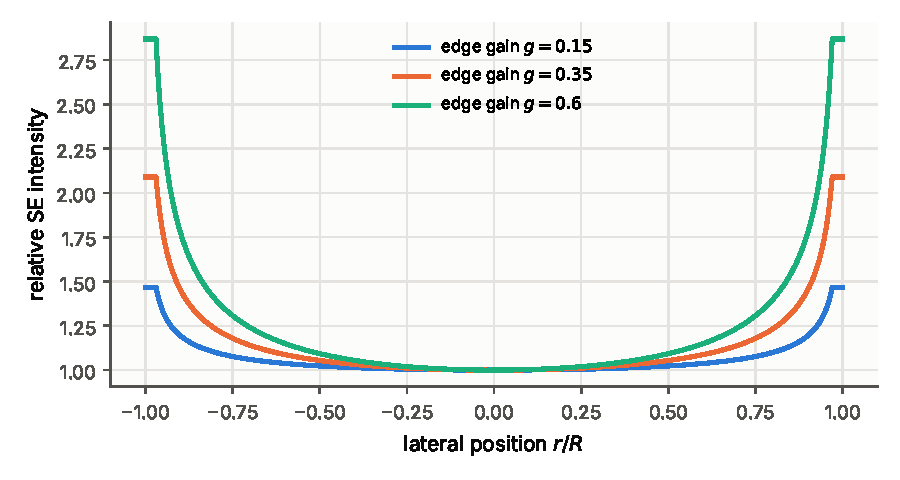
\includegraphics[width=0.62\linewidth]{figures/se_profile.pdf}
\caption{Cross-section intensity of a wire for three edge gains $g$ (secant law on a cylinder).}\label{fig:seprofile}
\end{figure}

\paragraph{Substrate and distractors.} The background is a random grey level with low-frequency fluctuations (Gaussian-filtered noise), fine grain and a linear charging gradient. With probability 0.25 dark pores of a filter membrane are added. With probability 0.5 Au nanoparticles are added. They are rendered with the same edge physics but are \emph{not} labelled as wires, so the network must learn to ignore them.

\paragraph{Acquisition.} With the ideal image $J$, the recorded image is
\begin{equation}
I = \Bigl[\tfrac1N\,\mathrm{Poisson}\bigl(N\,(J*G_{\sigma_b})\bigr)+\varepsilon_{\text{read}}+\eta_{\text{row}}\Bigr]^{\gamma},
\end{equation}
where $G_{\sigma_b}$ is the probe point-spread function (Gaussian, $\sigma_b\in[0.4,1.4]$\,px). $N\in[15,250]$ is the electron dose per unit intensity, which gives a signal-to-noise ratio $\mathrm{SNR}=\sqrt{NJ}$. $\varepsilon_{\text{read}}$ is Gaussian read noise, $\eta_{\text{row}}$ a random offset per scan line, and $\gamma\in[0.8,1.25]$ a detector non-linearity. With probability 0.3 the image is JPEG re-compressed at quality 40--95, since colleagues often save micrographs as JPEG. Finally, the same robust normalisation as for real images is applied (Section~\ref{sec:io}).

\subsection{Dense three-dimensional meshes (in-lens look)}\label{sec:dense3d}
Real AuNW meshes are often thick, three-dimensional stacks imaged with an in-lens detector at low voltage (e.g.\ 1\,kV). Compared with wires on a substrate they differ in four ways, each modelled explicitly in the \code{dense3d} style (65\,\% of all training images):
\begin{enumerate}[leftmargin=*,itemsep=1pt]
\item \textbf{Depth.} Wires are distributed over $L\in[3,6]$ layers. Layer $l$ ($0$ = deepest) has brightness
\begin{equation}
b_l=b_{\text{top}}\Bigl[\delta+(1-\delta)\Bigl(\tfrac{l}{L-1}\Bigr)^{\gamma}\Bigr],\qquad \delta\in[0.25,0.6],
\end{equation}
because fewer secondary electrons escape from deeper in the stack. After each layer the image rendered so far is blurred with $G_{\sigma_l}$; since Gaussians compose, layer $l$ ends up blurred with $\sigma_{\text{eff},l}=(\sum_{k\ge l}\sigma_k^2)^{1/2}$. This is the limited depth of field. Optionally the deepest layer is an unlabelled ``texture'' of very blurred wires.
\item \textbf{Shading.} Every wire darkens what lies below it by $1-h\,e^{-(d-R)/\lambda}$ next to its edge ($h$ up to 0.45).
\item \textbf{Faceted ribbons.} Pentagonally twinned wires look like flat ribbons with longitudinal facets. With the signed lateral coordinate $n$, the profile is multiplied by $1+f\cos(2.4\,k(n)+\varphi)$, where $k(n)=\lfloor(n/w+\tfrac12)\,K\rfloor$ is the facet index ($K=2,3$). A dark outline $1-o\,e^{-((R-d)/0.9)^2}$ and fine transverse striations $1+a\sin(2\pi s/(\Lambda w)+\psi)$ along the arc length $s$ (period $\Lambda w$ with $\Lambda\in[0.08,0.3]$) complete the look.
\item \textbf{Density, length and noise.} 3--9 wires per layer and $256^2$ tile, coverage typically 50--100\,\%, median length 150--900\,px (most wires cross the field), and long dwell times, i.e.\ low noise (log-uniform dose $N\in[30,1500]$).
\end{enumerate}
Figure~\ref{fig:dense} compares a real micrograph with synthetic images of this style.

\begin{figure}[H]\centering
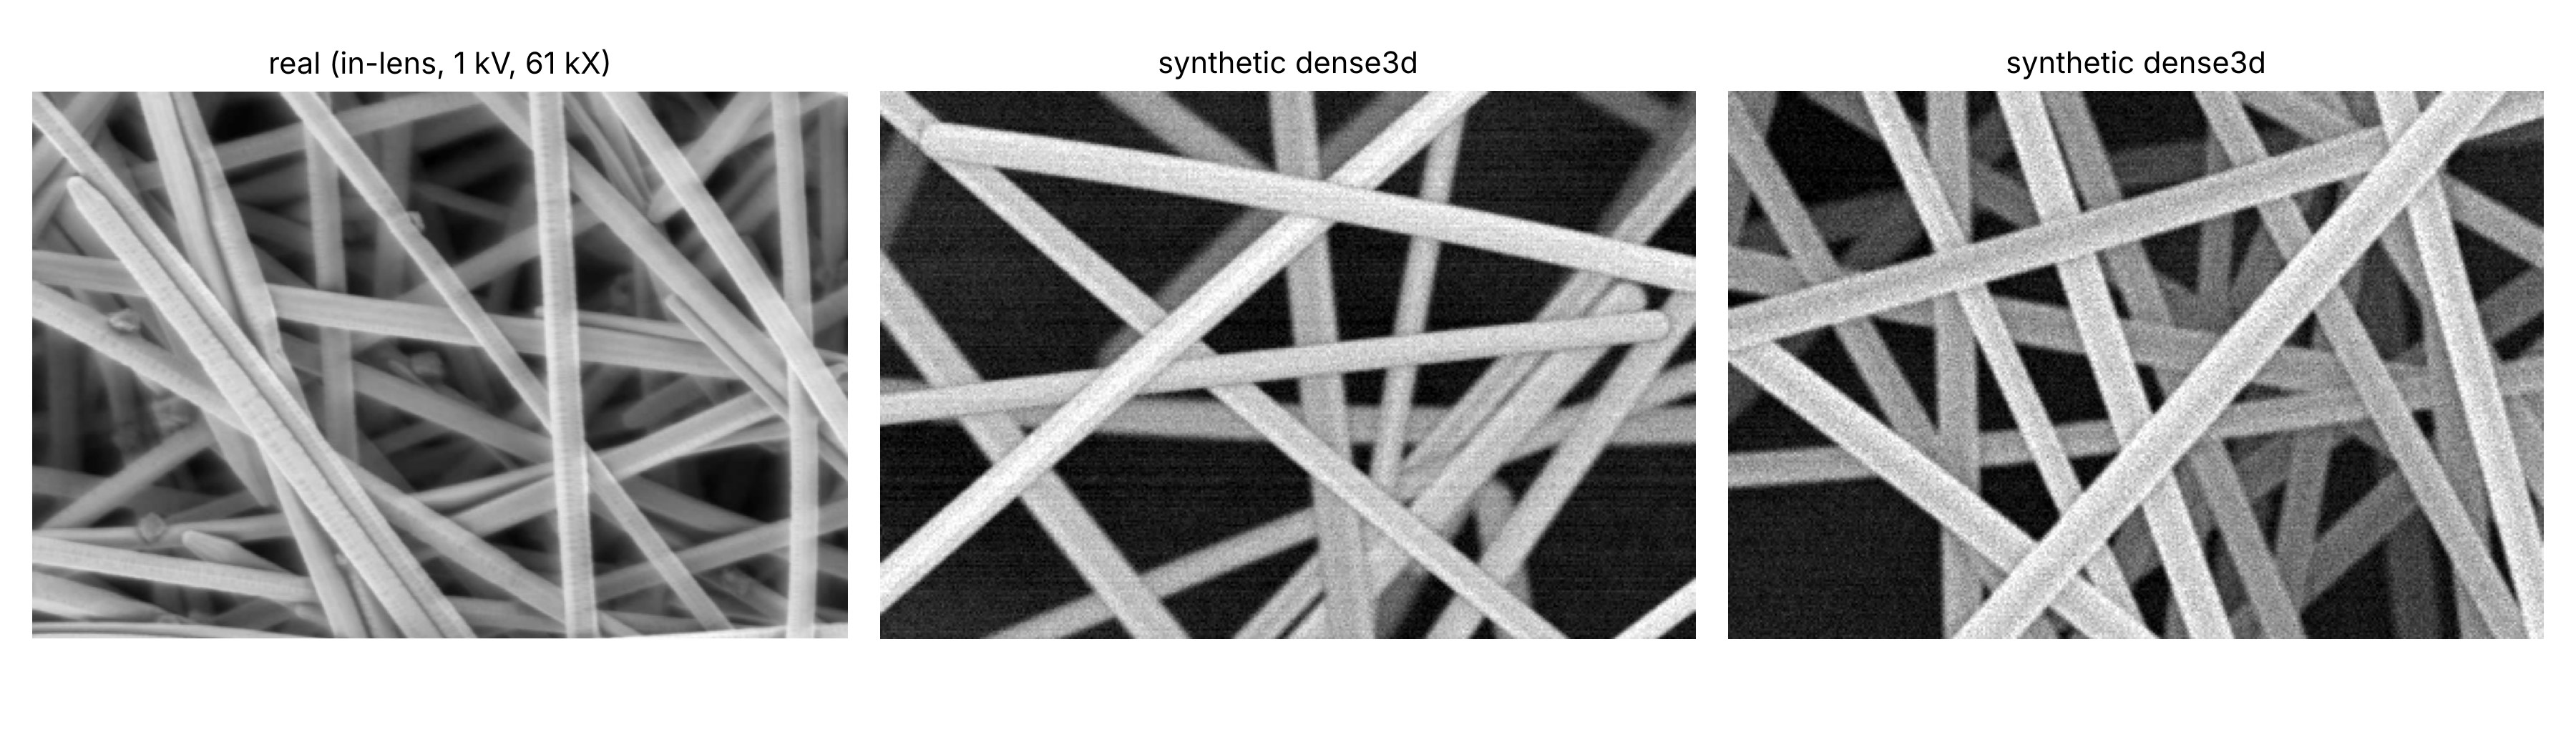
\includegraphics[width=\linewidth]{figures/real_vs_synthetic.jpg}
\caption{Left: real micrograph (in-lens, 1\,kV, 61\,kX). Right: synthetic \code{dense3d} images rendered by the generator at a similar wire width.}\label{fig:dense}
\end{figure}

\paragraph{Domain randomisation.} Every one of these parameters is drawn anew for every image. The network therefore sees a \emph{distribution} of imaging conditions that contains real microscopes as plausible samples, and it is forced to learn the invariant: the shape of a wire. Figure~\ref{fig:synth} shows examples with their labels.

\begin{figure}[H]\centering
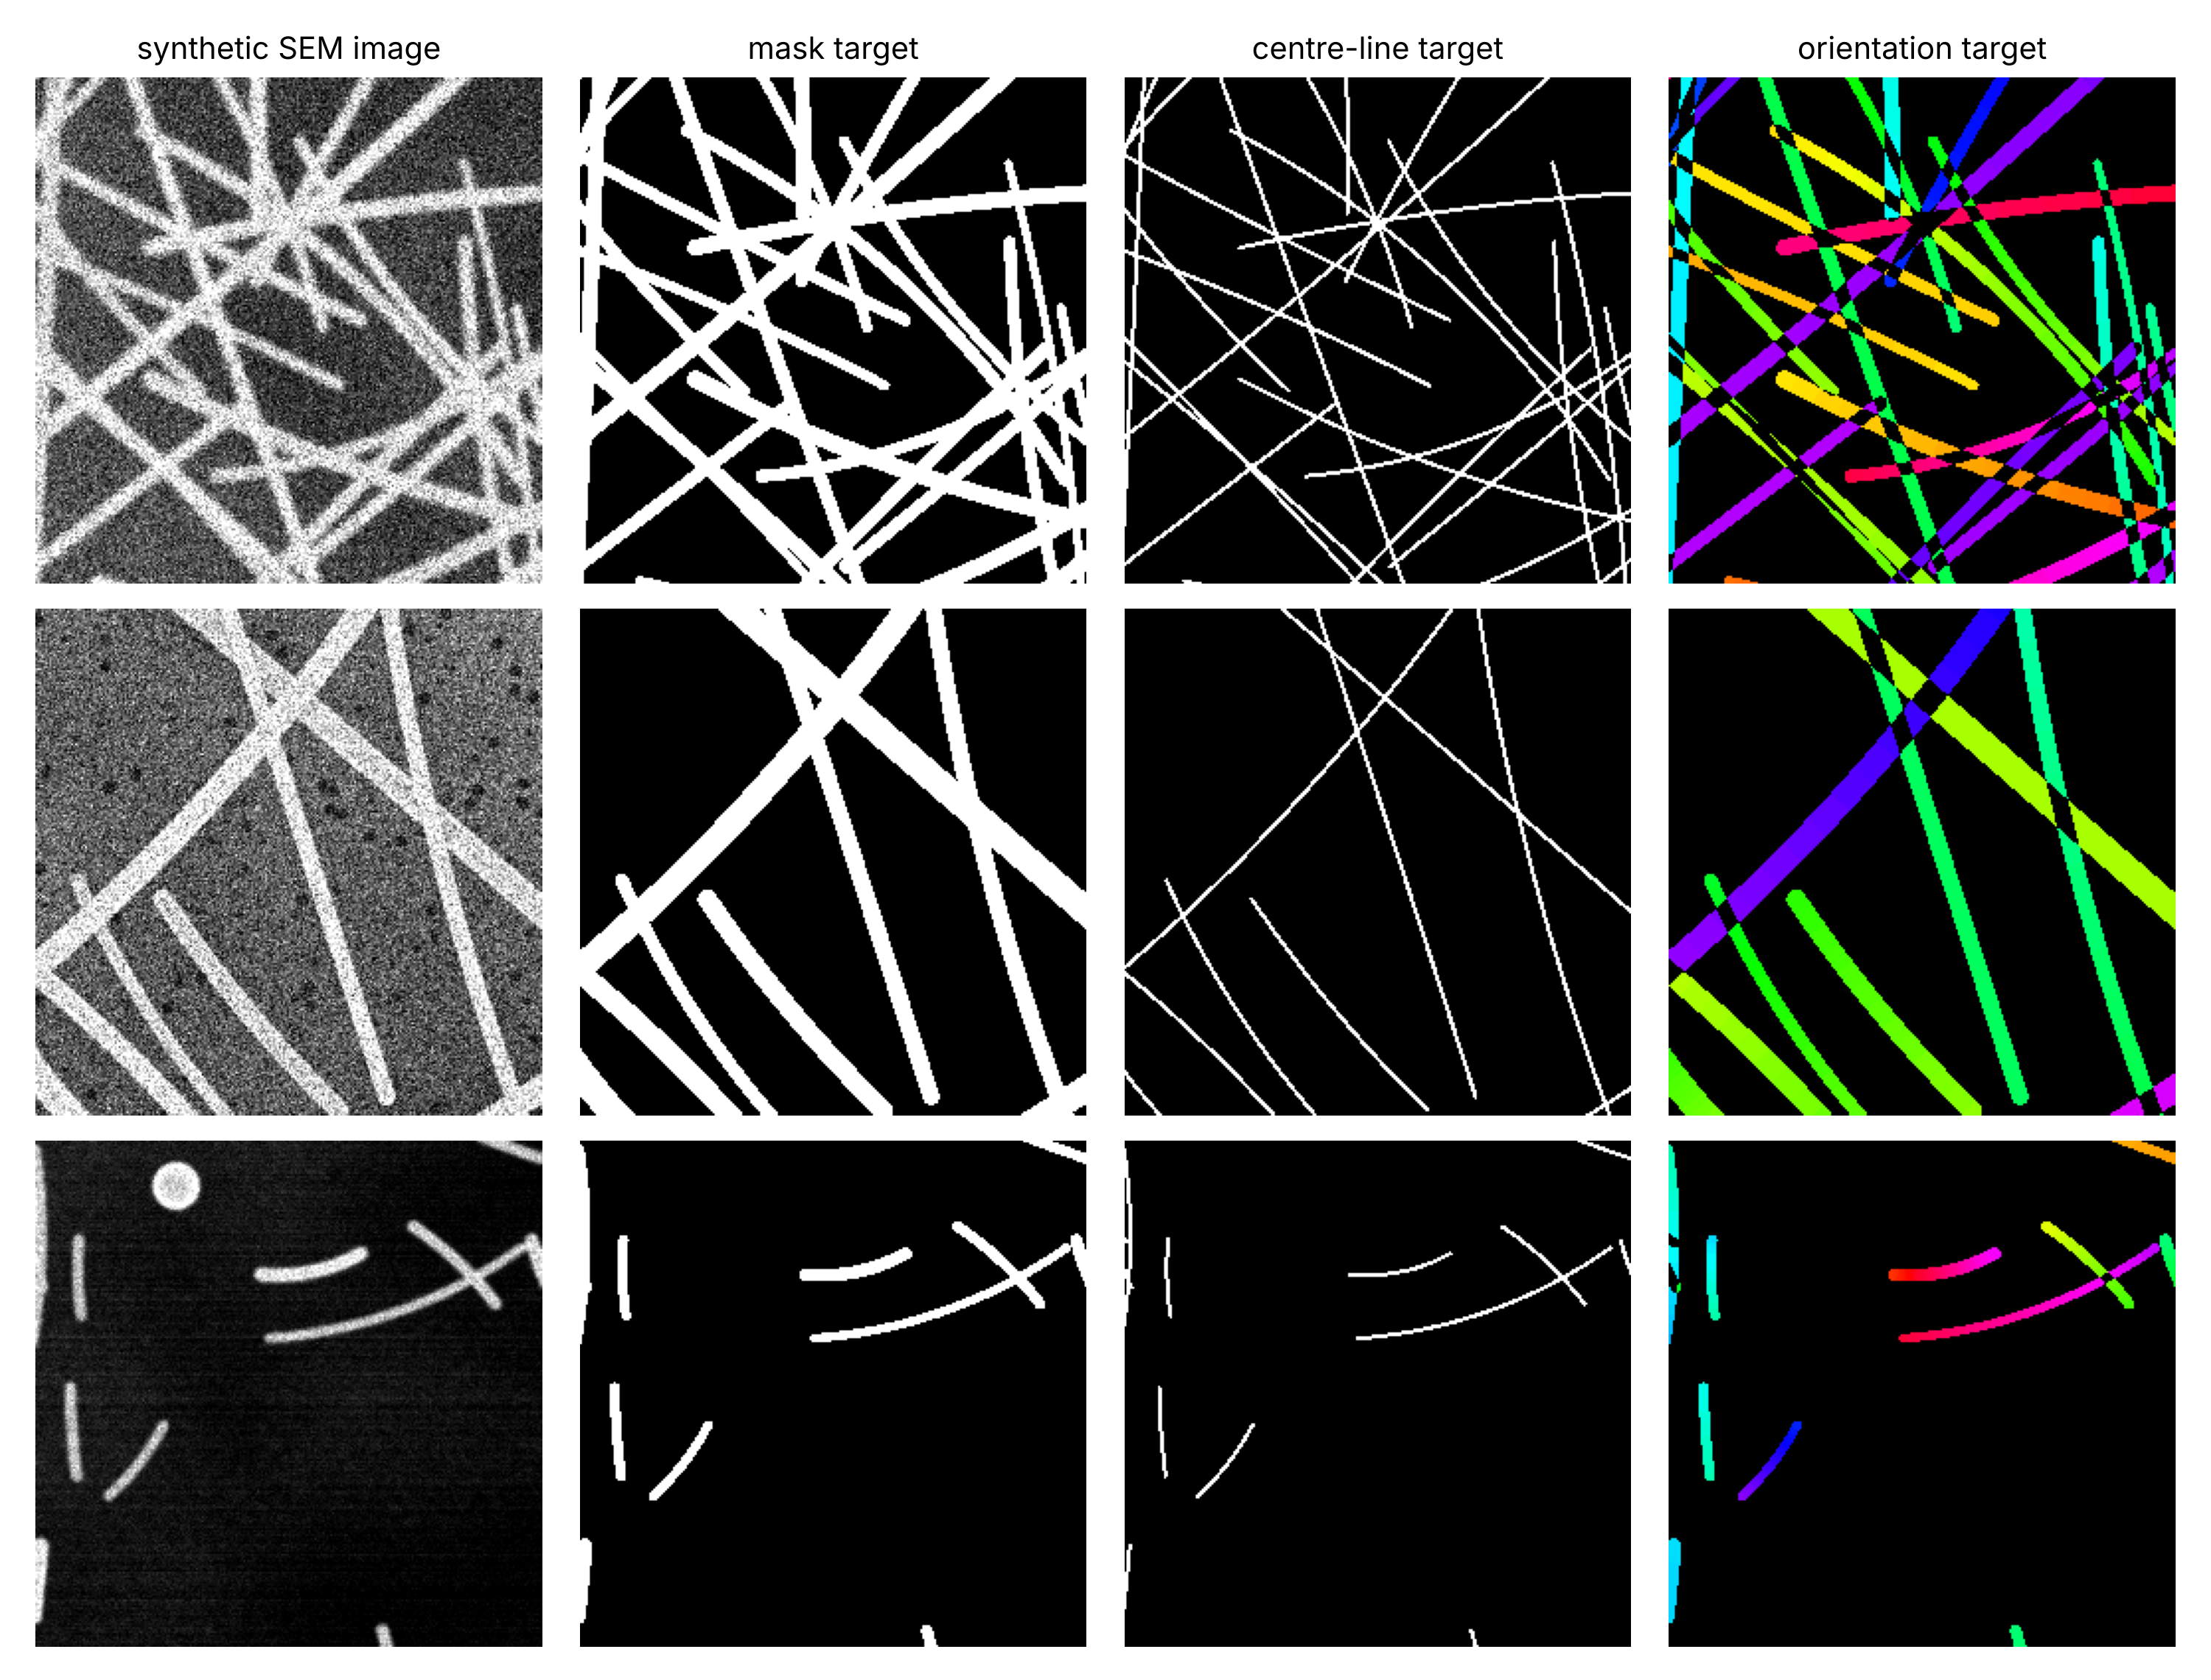
\includegraphics[width=0.95\linewidth]{figures/synthetic_examples.png}
\caption{Synthetic training tiles and their exact labels. Orientation is colour-coded by hue; black marks pixels without a reliable orientation (background and crossings).}\label{fig:synth}
\end{figure}

%==========================================================================
\section{Learning targets and data pipeline}\label{sec:targets}
%==========================================================================
For every training tile four targets are stored (\code{dataset.py}). All of them describe what is \emph{visible}, i.e.\ the top-most wire at each pixel:
\begin{description}[leftmargin=1.2em,itemsep=1pt]
\item[Mask] $y_m(\mathbf x)=1$ if any wire covers $\mathbf x$ ($a\ge\tfrac12$).
\item[Centre-line] $y_c(\mathbf x)=1$ if $d(\mathbf x)\le1$\,px for the \emph{visible} wire, a 3-px wide line. The upper wire of a crossing hides the centre-line of the lower one, whose centre-line is therefore interrupted; the measurement bridges such gaps (Section~\ref{sec:graph}). An earlier version also labelled the hidden parts. In thick meshes that asks the network for the impossible (centre-lines of wires buried under several others): it produced blurred maps, and even on \emph{perfect} labels the graph then recovered only 33\,\% of each wire as one piece, against 76\,\% with visible-only labels.
\item[Orientation] The wire axis is an \emph{axial} quantity: $\theta$ and $\theta+\pi$ describe the same wire. Regressing $\theta$ directly would create an artificial discontinuity at $0^\circ/180^\circ$. We therefore use the double-angle representation
\begin{equation}
\mathbf o=(\cos2\theta,\sin2\theta)\in S^1,
\end{equation}
which is continuous and unique for axial data. The prediction $\hat{\mathbf o}$ gives $\hat\theta=\tfrac12\operatorname{atan2}(\hat o_2,\hat o_1)$ and a confidence $|\hat{\mathbf o}|$. The squared error relates to the angle error $\Delta\theta$ by
\begin{equation}
\|\mathbf o-\hat{\mathbf o}\|^2 = 2-2\cos 2\Delta\theta = 4\sin^2\Delta\theta \approx 4\Delta\theta^2 .
\end{equation}
The orientation of the top-most wire is used; a weight $\mu(\mathbf x)=0$ excludes the background from the loss.
\item[Width] $y_w(\mathbf x)=w$ of the top-most wire (in px), stored in steps of $\tfrac14$\,px. In a dense mesh the wire mask is one connected area, so the width cannot be read from mask edges: a cross-section of the mask runs straight into the touching neighbour. A per-pixel width map does not have this problem.
\end{description}

\paragraph{Label-consistent augmentation.} Random flips and $90^\circ$ rotations multiply the effective data by 8. They must be applied to the orientation \emph{vector}, not only to the pixel grid. A horizontal or vertical flip maps $\theta\mapsto-\theta \pmod\pi$, hence $(o_1,o_2)\mapsto(o_1,-o_2)$. A rotation by $90^\circ$ maps $\theta\mapsto\theta+\pi/2$, hence $2\theta\mapsto2\theta+\pi$ and $(o_1,o_2)\mapsto(-o_1,-o_2)$. These sign rules are implemented in \code{\_augment} and verified by a unit test that compares the transformed label with the principal axis of the transformed mask. Photometric augmentation (contrast, brightness, gamma, Gaussian noise) acts only on the input.

\paragraph{Pipeline.} \code{tf.data.Dataset.from\_tensor\_slices} $\to$ \code{map} (targets) $\to$ \code{shuffle} $\to$ \code{map} (augmentation, parallel) $\to$ \code{batch} $\to$ \code{prefetch}. Augmentation runs on the CPU in parallel with the training step on the accelerator. The validation set is rendered with a different random seed and is never augmented.

%==========================================================================
\section{Network architecture}\label{sec:net}
%==========================================================================
\begin{figure}[H]\centering
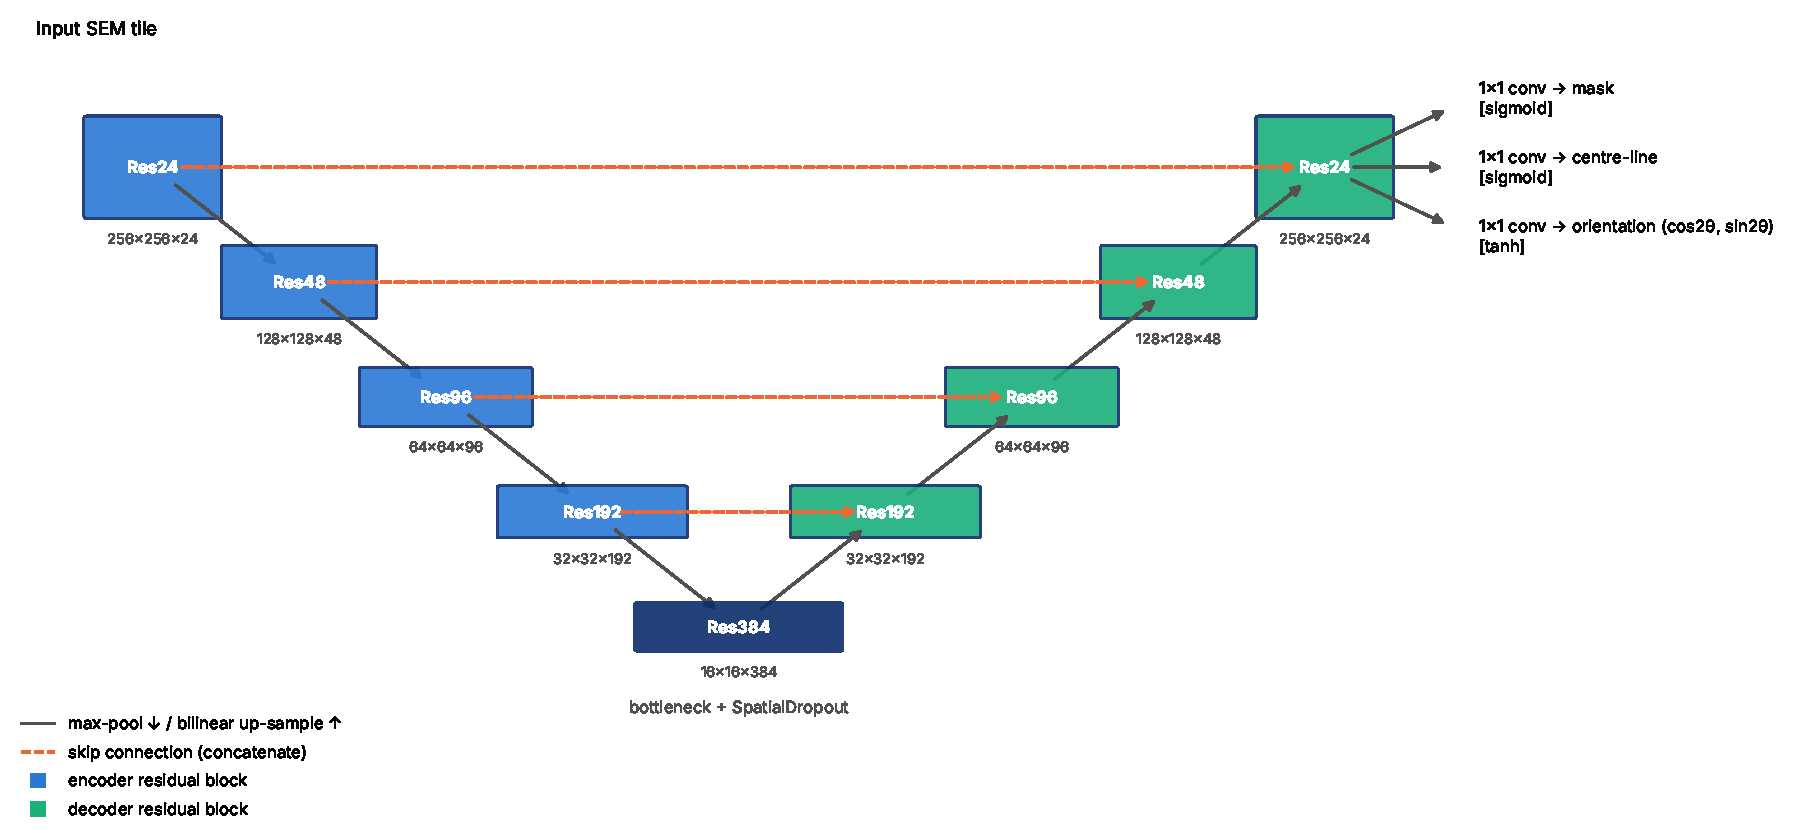
\includegraphics[width=\linewidth]{figures/unet.pdf}
\caption{Residual U-Net (default configuration: base 24 filters, depth 4). Box height $\propto$ resolution, label = output shape.}\label{fig:unet}
\end{figure}

\subsection{Residual U-Net}
The U-Net~\cite{ronneberger2015} is the standard architecture for dense prediction when training data are limited. An \emph{encoder} halves the resolution four times while doubling the channels ($24\to48\to96\to192\to384$), so it learns increasingly abstract and spatially extended features. A \emph{decoder} restores full resolution. \emph{Skip connections} concatenate encoder features of equal resolution into the decoder, restoring the precise edge positions lost by pooling, which is essential for measuring widths. Each block is a residual block~\cite{he2016}:
\begin{equation}
\mathbf y=\mathrm{ReLU}\Bigl(\mathrm{BN}\bigl(W_2*\mathrm{ReLU}(\mathrm{BN}(W_1*\mathbf x))\bigr)+P\mathbf x\Bigr),
\end{equation}
with $3\times3$ convolutions $W_{1,2}$ and $P$ either the identity or a $1\times1$ projection when the channel count changes. The identity path gives gradients a short route through the network and eases optimisation. Batch normalisation,
$\mathrm{BN}(x)=\gamma\,(x-\mu_B)/\sqrt{\sigma_B^2+\epsilon}+\beta$,
stabilises training and acts as a mild regulariser. Convolutions before BN carry no bias, because BN's $\beta$ makes it redundant. A convolution has $k^2C_{\text{in}}C_{\text{out}}$ weights; the default network has $4.67$\,M parameters, and the CPU preset (16 base filters) has $2.08$\,M.

\paragraph{Up-sampling.} Bilinear up-sampling followed by convolution is used instead of transposed convolutions. Transposed convolutions with stride 2 produce checkerboard artefacts~\cite{odena2016}, a periodic bias of edge positions that would translate directly into width errors.

\paragraph{Receptive field.} With kernel size $k$ and cumulative stride (``jump'') $j$, each layer enlarges the receptive field by $r\leftarrow r+(k-1)j$, and pooling multiplies the jump: $j\leftarrow 2j$. Summing over the encoder, bottleneck and decoder (\code{receptive\_field}) gives
\begin{equation}
r = 1+\sum_{\ell=0}^{3}\bigl(4\cdot2^\ell+2^\ell\bigr)+4\cdot 16+\sum_{\ell=0}^{3}4\cdot2^\ell = 200\ \text{px}.
\end{equation}
At the target wire width of about 9\,px (Section~\ref{sec:autoscale}), one output pixel therefore sees more than 20 wire widths. That is enough context to see both arms of a crossing and to decide which centre-line continues where.

\paragraph{Four heads.} Four $1\times1$ convolutions on the last decoder features give
$p_m=\sigma(\cdot)$, $p_c=\sigma(\cdot)$, $\hat{\mathbf o}=\tanh(\cdot)\in(-1,1)^2$ and the width $\hat w=\operatorname{softplus}(\cdot)=\ln(1+e^{(\cdot)})>0$. The heads share all features (multi-task learning). The orientation task forces the shared features to encode direction, which also helps the centre-line head at crossings. The heads are computed in float32 even under mixed precision.

\subsection{Loss functions}
For a binary map with targets $y_i$ and predictions $p_i$ over the $N$ pixels of a tile,
\begin{align}
\mathcal L_{\text{BCE}}&=-\frac1N\sum_i\bigl[y_i\ln p_i+(1-y_i)\ln(1-p_i)\bigr],\\
\mathcal L_{\text{Dice}}&=1-\frac{2\sum_i y_ip_i+\epsilon}{\sum_iy_i+\sum_ip_i+\epsilon},
\end{align}
and the mask and centre-line heads use $\mathcal L_{\text{BCE}}+\mathcal L_{\text{Dice}}$. BCE yields calibrated probabilities, which matters because the width is measured at $p_m=\tfrac12$. The Dice term is invariant to class imbalance; the centre-lines cover only a few percent of the pixels, and with BCE alone the trivial prediction ``no centre-line'' would already have a low loss. The orientation loss is the weighted squared error
\begin{equation}
\mathcal L_{\text{o}}=\frac{\sum_i\mu_i\,\|\mathbf o_i-\hat{\mathbf o}_i\|^2}{\sum_i\mu_i+1},
\end{equation}
the width loss is the weighted \emph{relative} error, which gives thin and thick wires equal importance,
\begin{equation}
\mathcal L_{\text{w}}=\frac{\sum_i m_i\,|\hat w_i-w_i|/\max(w_i,1)}{\sum_i m_i+1}\qquad(m_i=1\text{ on wire pixels}),
\end{equation}
and the total loss is $\mathcal L=\mathcal L_m+\mathcal L_c+0.5\,\mathcal L_o+0.5\,\mathcal L_w$. Monitored metrics are the hard Dice coefficient (F1 score) at threshold $0.5$ for mask and centre-line, and the mean axial angle error $\overline{\min(|\Delta\theta|,\pi-|\Delta\theta|)}$.

%==========================================================================
\section{Training and the control of over-fitting}\label{sec:training}
%==========================================================================
\subsection{Optimiser}
AdamW~\cite{loshchilov2019} with gradient $g_t$:
\begin{align}
m_t&=\beta_1m_{t-1}+(1-\beta_1)g_t,\qquad v_t=\beta_2v_{t-1}+(1-\beta_2)g_t^2,\\
\theta_t&=\theta_{t-1}-\eta_t\Bigl(\frac{\hat m_t}{\sqrt{\hat v_t}+\epsilon}+\lambda\,\theta_{t-1}\Bigr),\quad \hat m_t=\frac{m_t}{1-\beta_1^t},\ \hat v_t=\frac{v_t}{1-\beta_2^t}.
\end{align}
The weight decay $\lambda=10^{-4}$ is \emph{decoupled} from the adaptive gradient scaling. Classical $L_2$ regularisation added to the loss would be divided by $\sqrt{\hat v_t}$, so parameters with large gradients would be regularised less, which is the opposite of the intent. Gradients are clipped to norm 1 for robustness against rare outlier batches. The start learning rate is $\eta_0=10^{-3}$.

\subsection{Countermeasures against over-fitting}
Over-fitting means that the training loss keeps decreasing while the loss on unseen data rises: the network memorises the training samples instead of the underlying regularity. The following measures act at different levels:
\begin{enumerate}[leftmargin=*,itemsep=1pt]
\item \textbf{Independent validation set} from a different generator seed (and, for real data, from \emph{different images}; Section~\ref{sec:finetune}). This is the only honest estimate of the generalisation error.
\item \textbf{Early stopping} with restoration of the best weights: with $t^*=\arg\min_{t'\le t}\mathcal L_{\text{val}}(t')$, training stops when $t-t^*\ge P$ ($P=10$), and the weights of epoch $t^*$ are restored. This is equivalent to choosing the training length by validation.
\item \textbf{Learning-rate reduction} on a plateau: $\eta\leftarrow\eta/2$ after 4 epochs without improvement. A smaller step size often resolves an apparent plateau and gives a better minimum before early stopping triggers.
\item \textbf{Capacity regularisation}: decoupled weight decay, \code{SpatialDropout2D} (rate 0.15) in the two deepest levels and the bottleneck, where most parameters are, and BatchNorm. SpatialDropout drops whole feature maps rather than single activations, because neighbouring activations in a conv layer are strongly correlated and ordinary dropout would hardly regularise them.
\item \textbf{Data augmentation} (Section~\ref{sec:targets}) and the practically unlimited synthetic data.
\end{enumerate}

\paragraph{Transfer learning.} When the architecture grows (as with the added width head), training does not start from random weights. All layers whose name and weight shapes agree are copied from the previous network (\code{transfer\_weights}), and only the new layers start from scratch. The dense-mesh network was obtained this way from the first network in two stages.

\paragraph{Training as a separate process.} The GUI does not train inside its own process. It launches the same command a user could type (\code{python -m aunw.cli train \dots}) as a separate process, which writes its progress to \code{progress.json} and \code{preview.npz} in the model folder; the GUI only reads these files. A stop request is a file \code{STOP}, which the trainer checks after every batch, keeping the best weights. This design means that a crash in the numerical libraries can never take down the user interface (an early threaded version did exactly that inside the web server). It also means that training continues when the browser is closed, and that every GUI run is reproducible from the command shown on screen.

\paragraph{Monitoring.} The GUI (step 3) and TensorBoard show the per-batch loss, all per-epoch metrics for training and validation, the learning rate, and predictions on fixed validation tiles after every epoch. In addition, \code{overfitting\_report} computes the generalisation gap
\begin{equation}
\Delta_t=\mathcal L_{\text{val}}(t)-\mathcal L_{\text{train}}(t)
\end{equation}
and raises an over-fitting flag when $\mathcal L_{\text{val}}$ has risen over the last 3 epochs while $\mathcal L_{\text{train}}$ fell. Note that $\Delta_t$ can be negative early in training: training metrics are averaged over an epoch with dropout active and with augmented samples, whereas validation is evaluated at the end of the epoch, in inference mode, on unaugmented data.

%==========================================================================
\section{Inference on full SEM images}\label{sec:inference}
%==========================================================================
\subsection{Pre-processing}\label{sec:io}
Images are converted to grey (luminance for RGB) and normalised robustly:
$I\leftarrow\mathrm{clip}\bigl((I-q_{0.5})/(q_{99.5}-q_{0.5}),0,1\bigr)$, with $q_p$ the $p$-th percentile. Percentiles instead of minimum/maximum make the result insensitive to hot pixels and to the 16-bit range of many SEM TIFFs. The instrument information bar is detected as a block of rows that are mostly saturated, then cropped; the value can be corrected in the GUI. The pixel size is read from FEI/Thermo Fisher metadata (\code{PixelWidth}, in metres), Zeiss SmartSEM metadata (\code{Image Pixel Size}) or ImageJ calibration. It can also be entered by hand or computed from the scale bar as $s=\ell_{\text{bar}}[\mathrm{nm}]/\ell_{\text{bar}}[\mathrm{px}]$.

\subsection{Automatic scale selection}\label{sec:autoscale}
The network was trained on wires $\approx3$--$20$\,px wide. A real micrograph is therefore resized by a factor $s$ so that the median wire width is close to the target $w^\ast=9$\,px. Starting at $s_0=1$, a central crop is analysed and the median width $\hat w(s_n)$ measured; then
\begin{equation}
s_{n+1}=s_n\,\frac{w^\ast}{\hat w(s_n)},
\end{equation}
until $w^\ast/\hat w\in(0.75,1.33)$ (at most 3 iterations). Iteration is necessary because a network that sees wires far outside its training range under-estimates how wrong the scale is. All measurements are divided by $s$ afterwards.

\subsection{Tiled prediction with seamless blending}
The image is processed in tiles of $T=256$\,px with overlap $o=64$\,px (stride $T-o$). After reflective padding by $o$ on every side, the number of tiles along an axis of length $H$ is $n=\lceil(H+2o-T)/(T-o)\rceil+1$. Each tile prediction $f(T_k)$ is weighted by a window $\omega(\mathbf x)=\omega_1(x)\omega_1(y)$ that is 1 in the centre and decays as $\sin^2$ over the overlap. The blended prediction is
\begin{equation}
P(\mathbf x)=\frac{\sum_k\omega_k(\mathbf x)\,f(T_k)(\mathbf x)}{\sum_k\omega_k(\mathbf x)} .
\end{equation}
Tile borders, where convolutions see artificial padding, receive almost zero weight, so no seams appear. A unit test with an identity network verifies $P\equiv I$ to $10^{-5}$ for arbitrary image sizes.

\subsection{Test-time augmentation (TTA)}
With the flip group $\mathcal G=\{\mathrm{id},\text{LR},\text{UD},\text{LR}\circ\text{UD}\}$, the prediction is
$\bar P=\frac14\sum_{g\in\mathcal G}g^{-1}f(gI)$. Mask and centre-line maps are simply flipped back. For the orientation, a single flip reverses the sign of $o_2$, while the double flip (a $180^\circ$ rotation) leaves $\mathbf o$ unchanged. Averaging double-angle vectors is the correct axial mean. TTA reduces the variance of the prediction at four times the cost.

%==========================================================================
\section{Separating individual wires}\label{sec:graph}
%==========================================================================
\begin{figure}[H]\centering
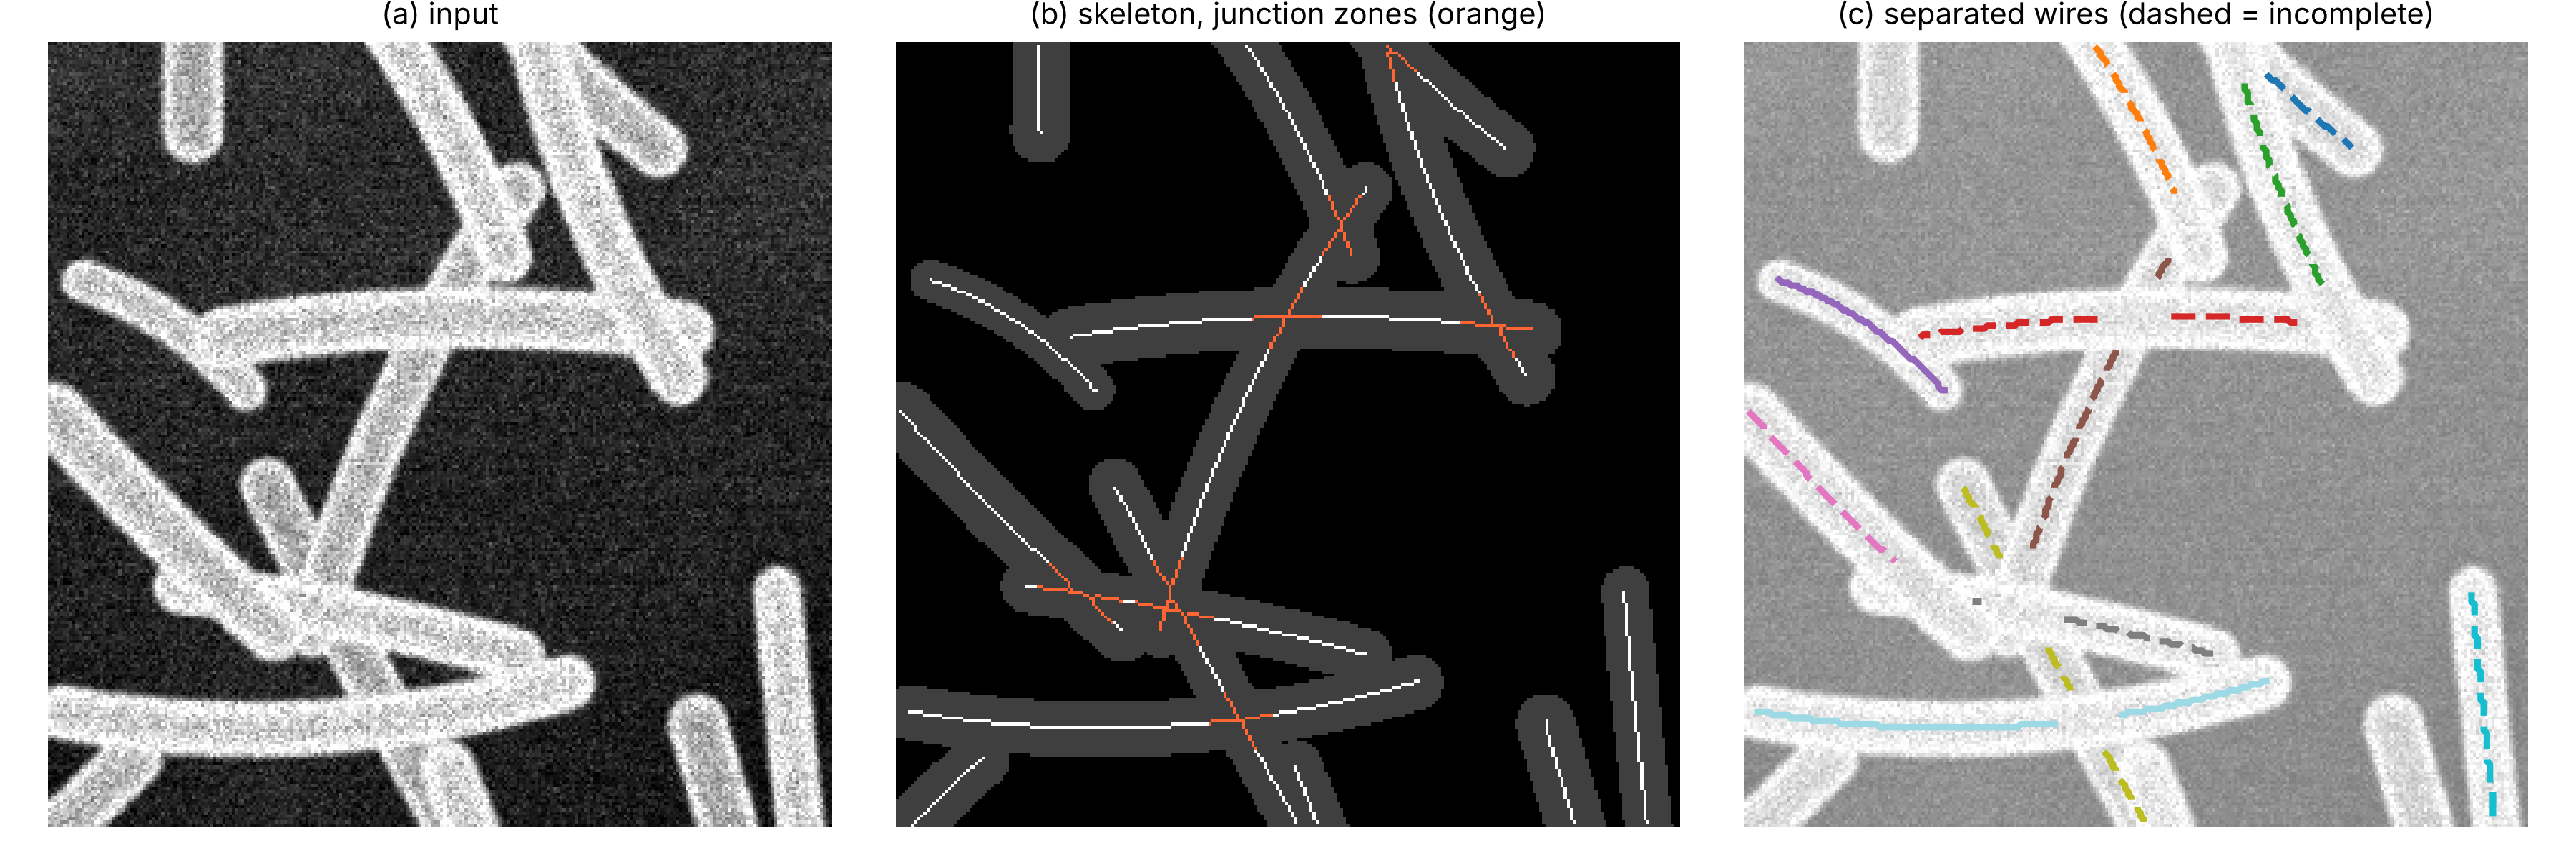
\includegraphics[width=\linewidth]{figures/graph_steps.png}
\caption{Wire separation on a synthetic tile. (b) Skeleton of the centre-line map with junction zones. (c) Wires after pairing branches through junctions; each colour is one physical wire.}\label{fig:graph}
\end{figure}

\subsection{Skeleton and junctions}
The centre-line map is thresholded inside the mask, $C=\{p_c>\tfrac12\}\cap\{p_m>\tfrac12\}$, and thinned to an 8-connected skeleton $S$ of one-pixel width. For a skeleton pixel with cyclically ordered neighbours $P_1,\dots,P_8$ ($P_9=P_1$), the \emph{crossing number}
\begin{equation}
\mathrm{CN}=\tfrac12\sum_{k=1}^{8}|P_{k+1}-P_k|
\end{equation}
counts the number of branches leaving the pixel: 1 at an end, 2 on a line, $\ge3$ at a junction. Unlike the neighbour count, CN does not create false junctions on staircase-shaped diagonal lines. Compact junction clusters, where every pixel individually has $\mathrm{CN}=2$, are caught by an additional neighbour count $\ge4$. Validation showed that 4\,\% of skeleton pixels were otherwise traced incorrectly. Junction pixels are dilated into \emph{junction zones} of radius $r_j=\lceil w/2\rceil+1$ (with $w$ the global width estimate $w\approx2\,\mathrm{EDT}-1$ on the skeleton). Removing the zones splits the skeleton into \emph{branches}, simple pixel chains. Each chain is ordered by walking from an end in both directions.

\subsection{Pairing branches through junctions}
For every branch end inside junction $j$ we compute an outward unit vector $\mathbf u$ pointing into the junction. Its axis comes from the axial mean of the orientation head over the last $m=\max(8,3w)$ pixels, when that is confident ($|\bar{\mathbf o}|>0.5$); its sign comes from the geometry. Two ends $a,b$ with tip separation $\mathbf r$ are candidates for one wire running straight through the junction if
\begin{align}
\delta_{ab}&=\arccos(-\mathbf u_a\cdot\mathbf u_b)<\delta_{\max}=25^\circ \quad\text{(deflection)},\\
\ell_{ab}&=\max\bigl(|\mathbf u_a\times\mathbf r|,|\mathbf u_b\times\mathbf r|\bigr)<\tau(|\mathbf r|)=\max(2,\tfrac w2)+0.1|\mathbf r| \quad\text{(collinearity)}.
\end{align}
The tolerance grows with the gap because a direction error $\epsilon$ produces a lateral offset $\approx\epsilon|\mathbf r|$. Candidates are accepted greedily in order of increasing cost $c_{ab}=\delta_{ab}/\delta_{\max}+\ell_{ab}/\tau$, with every end used at most once and no cycles. Accepted pairs are merged with a union--find structure; each resulting set of branches is one wire. The tolerance model was not guessed. It was chosen from logged statistics of true and false pairs on ground-truth maps: true continuations have a median lateral offset of 0.9\,px, false pairs 9\,px, and the fixed 2-px tolerance used initially rejected 22\,\% of true pairs.

\paragraph{Gap bridging.} Where two wires cross, the centre-line of the \emph{lower} wire can be interrupted, because the upper wire hides it. Its skeleton then ends in two facing free tips instead of a junction. Two free tips are therefore also linked when they are at most $4w+3$\,px apart (a crossing wire of width $w$ at angles down to about $30^\circ$) (candidates from a $k$-d tree), satisfy the same deflection and collinearity criteria, point towards each other ($\mathbf u_a\cdot\mathbf r>0$), and the straight segment between them lies entirely inside the wire mask ($\min p_m>\tfrac12$ along it), i.e.\ the wire visibly continues underneath.

\subsection{End classification and the ``complete'' flag}
Every unpaired end is classified as a \emph{tip} (a free end, not at the border, at which the wire mask ends as well), a \emph{T-end} (the only unpaired end in its junction: all other arms continue, so the wire ends on top of another wire), \emph{unresolved} (unpaired in a junction with other unpaired ends), or \emph{border}. A wire is \textbf{complete} if both ends are tips and it does not touch the border. Only then is its length fully observed. On ground truth, complete wires had a gross length error ($<-10\,\%$) in only $0.5\,\%$ of cases, against 26\,\% for wires with one T-end and 62\,\% with two. Length statistics therefore use complete wires; width statistics use all wires, because truncation does not affect width.

%==========================================================================
\section{Measurement}\label{sec:measure}
%==========================================================================
\subsection{Length}
A digital straight line at angle $\varphi\in[0^\circ,45^\circ]$ consists of $n_e=L(\cos\varphi-\sin\varphi)$ axial and $n_o=L\sin\varphi$ diagonal steps. The naive chain length is therefore
\begin{equation}
L_{\text{chain}}=n_e+\sqrt2\,n_o=L\bigl(\cos\varphi+(\sqrt2-1)\sin\varphi\bigr),
\end{equation}
which over-estimates $L$ by up to $\sqrt{4-2\sqrt2}-1=8.2\,\%$ at $\varphi=22.5^\circ$. We instead resample the ordered chain every $k=4$ pixels and sum the Euclidean polyline. With independent quantisation errors $\varepsilon\sim\mathcal U(-\tfrac12,\tfrac12)$ perpendicular to the line, $\mathrm{Var}(\Delta\varepsilon)=\tfrac16$ and
\begin{equation}
\frac{\E[L_{\text{poly}}]-L}{L}\approx\frac{\E[(\Delta\varepsilon)^2]}{2k^2}=\frac1{12k^2}=0.5\,\%\quad(k=4).
\end{equation}
The wire length is the sum of its branch lengths, the bridged junction gaps $|\mathbf r_{ab}|$, and end corrections. Each free end adds $w/2$, because the centre-line stops at the centre of the hemispherical cap, cf.\ Eq.~\eqref{eq:capsule}. An end inside a junction adds the distance to the junction centre, bounded by $r_j+w$.

\subsection{Width}
\paragraph{Primary: width map.} The width of a wire is the median of the predicted width map $\hat w$ along its centre-line, excluding junction neighbourhoods. Away from crossings the top-most wire at a centre-line pixel is the wire itself, so $\hat w$ there is its own width, even if neighbours touch it. A unit test checks two touching parallel wires, for which the edge-profile method below measures the double width.

\paragraph{Cross-check: sub-pixel edge profiles.} At every second centre-line pixel, at least one width away from tips and junctions, the mask probability is sampled along the local normal $\mathbf n$ (bilinear interpolation, step $\Delta t=0.25$\,px): $p(t)=p_m(\mathbf x+t\mathbf n)$. The edges are the first samples with $p\le\tfrac12$ on either side, refined by linear interpolation:
\begin{equation}
t_{\text{edge}}=t_{k-1}+\frac{p_{k-1}-\tfrac12}{p_{k-1}-p_k}\,\Delta t,\qquad w_i=t_{\text{edge}}^{+}+t_{\text{edge}}^{-}.
\end{equation}
The $\tfrac12$ level is the natural edge criterion: a step edge convolved with any symmetric point-spread function crosses $\tfrac12$ exactly at the true edge, and a calibrated posterior equals $\tfrac12$ at the decision boundary. The wire width is the \emph{median} of all $w_i$, which is robust to the outliers caused by touching neighbours and particles. If fewer than 3 profiles are valid, the distance-transform estimate $2\,\mathrm{EDT}-1$ is used. This value is exported as \code{width\_profile\_px}; it is exact for isolated wires.

%==========================================================================
\section{Statistics}\label{sec:stats}
%==========================================================================
For a sample $x_1,\dots,x_n$ the software reports the mean $\bar x$, the standard deviation $s$, the SEM $s/\sqrt n$ and the 95\,\% confidence interval $\bar x\pm t_{0.975,n-1}\,s/\sqrt n$. It also reports the median with a bootstrap 95\,\% interval (2.5 and 97.5 percentiles of the median over $B=2000$ resamples), the quartiles and the coefficient of variation $100\,s/\bar x$.

\paragraph{Log-normal model.} Nanowire lengths are typically right-skewed and well described by $\ln X\sim\mathcal N(\mu,\sigma^2)$. The maximum-likelihood estimates are $\hat\mu=\overline{\ln x}$ and $\hat\sigma^2=\overline{(\ln x-\hat\mu)^2}$, with median $e^{\hat\mu}$, mean $e^{\hat\mu+\hat\sigma^2/2}$, geometric mean $e^{\hat\mu}$ and geometric SD $e^{\hat\sigma}$. Normal and log-normal models are compared with the Akaike information criterion, $\mathrm{AIC}=2k-2\ln\hat{\mathcal L}$ (with $k=2$ for both); the model with the lower AIC is reported. Histograms use the Freedman--Diaconis bin width $h=2\,\mathrm{IQR}\,n^{-1/3}$.

\paragraph{Edge correction (Miles--Lantuéjoul).} A wire with bounding box $\Delta x\times\Delta y$, placed uniformly at random, lies completely inside a $W\times H$ frame with probability
\begin{equation}
\pi_i=\frac{(W-\Delta x_i)(H-\Delta y_i)}{WH}.
\end{equation}
Long wires are therefore under-represented among complete wires. Weighting each complete wire by $1/\pi_i$ (Horvitz--Thompson/Hájek estimator, $\bar x_w=\sum w_ix_i/\sum w_i$) removes this bias~\cite{miles1978,lantuejoul1980}. The weighted standard error uses the Kish effective sample size $n_{\text{eff}}=(\sum w_i)^2/\sum w_i^2$.

\paragraph{Stereological mean length.} An independent estimate of the mean length needs no wire separation at all. Consider a stationary random system of wires with number density $\lambda$ (wires per area) and mean length $\langle L\rangle$. A window of area $A$ contains on average $2\lambda A$ wire ends and a total wire length of $\lambda A\langle L\rangle$, irrespective of how many wires are cut by the frame. Hence
\begin{equation}
\widehat{\langle L\rangle}=\frac{2\,\Lambda}{N_{\text{ends}}},
\end{equation}
with $\Lambda$ the total measured wire length in the window and $N_{\text{ends}}$ the number of visible ends (free tips and T-ends; ends caused by unresolved crossings and border ends are excluded). The estimator is insensitive to pairing errors, because splitting a wire changes neither $\Lambda$ nor the number of true ends. It is reported per image next to the mean of the complete wires; agreement of the two is a practical consistency check.

\paragraph{Reliability classes by areal coverage.} The fraction $\phi$ of the image covered by wires determines how many wire ends are hidden under other wires. Each image is classified as \emph{good} ($\phi\le0.30$), \emph{caution} ($0.30<\phi\le0.45$) or \emph{length unreliable} ($\phi>0.45$). Width statistics stay reliable in all classes (Section~\ref{sec:validation}).

\paragraph{Comparing populations.} To compare automatic and manual measurements, or two samples, the software reports the two-sample Kolmogorov--Smirnov test $D=\sup_x|F_1(x)-F_2(x)|$ (shape), the Mann--Whitney $U$ test (location, non-parametric) and Welch's $t$ test (means, unequal variances), together with the relative differences of means and medians.

%==========================================================================
\section{Validation}\label{sec:validation}
%==========================================================================
Two levels are validated separately, because they fail for different reasons.

\paragraph{(1) The measurement algorithm alone.} The graph and measurement stages were run on \emph{perfect} maps, i.e.\ the ground-truth labels, for eight dense synthetic $768^2$ images, about 130--400 wires each. These numbers are the best the algorithm can do, independent of the network:

\begin{table}[H]\centering\small
\begin{tabular}{@{}lr@{}}\toprule
Complete wires: median relative length error & $+0.7\,\%$\\
Complete wires: length error within $\pm10\,\%$ / $\pm20\,\%$ & $91\,\%$ / $95\,\%$\\
All matched wires: median relative width error & $+0.65\,\%$\\
Single straight wire, four angles (unit test) & length $<3\,\%$, width $<5\,\%$\\\bottomrule
\end{tabular}
\end{table}

\paragraph{(2) The complete chain with the trained network (stage 1).} The first network (16 base filters, 2.1\,M parameters, trained on substrate-style images only) was trained on 1600 synthetic tiles for 35 epochs on 4 CPU cores (about 2\,h). Training and validation loss decreased together (Fig.~\ref{fig:curves}): there was no over-fitting, and the best validation loss was reached in the last epoch. A longer run on a GPU, or the larger default network (24 filters), can therefore be expected to improve the results further.

\begin{figure}[H]\centering
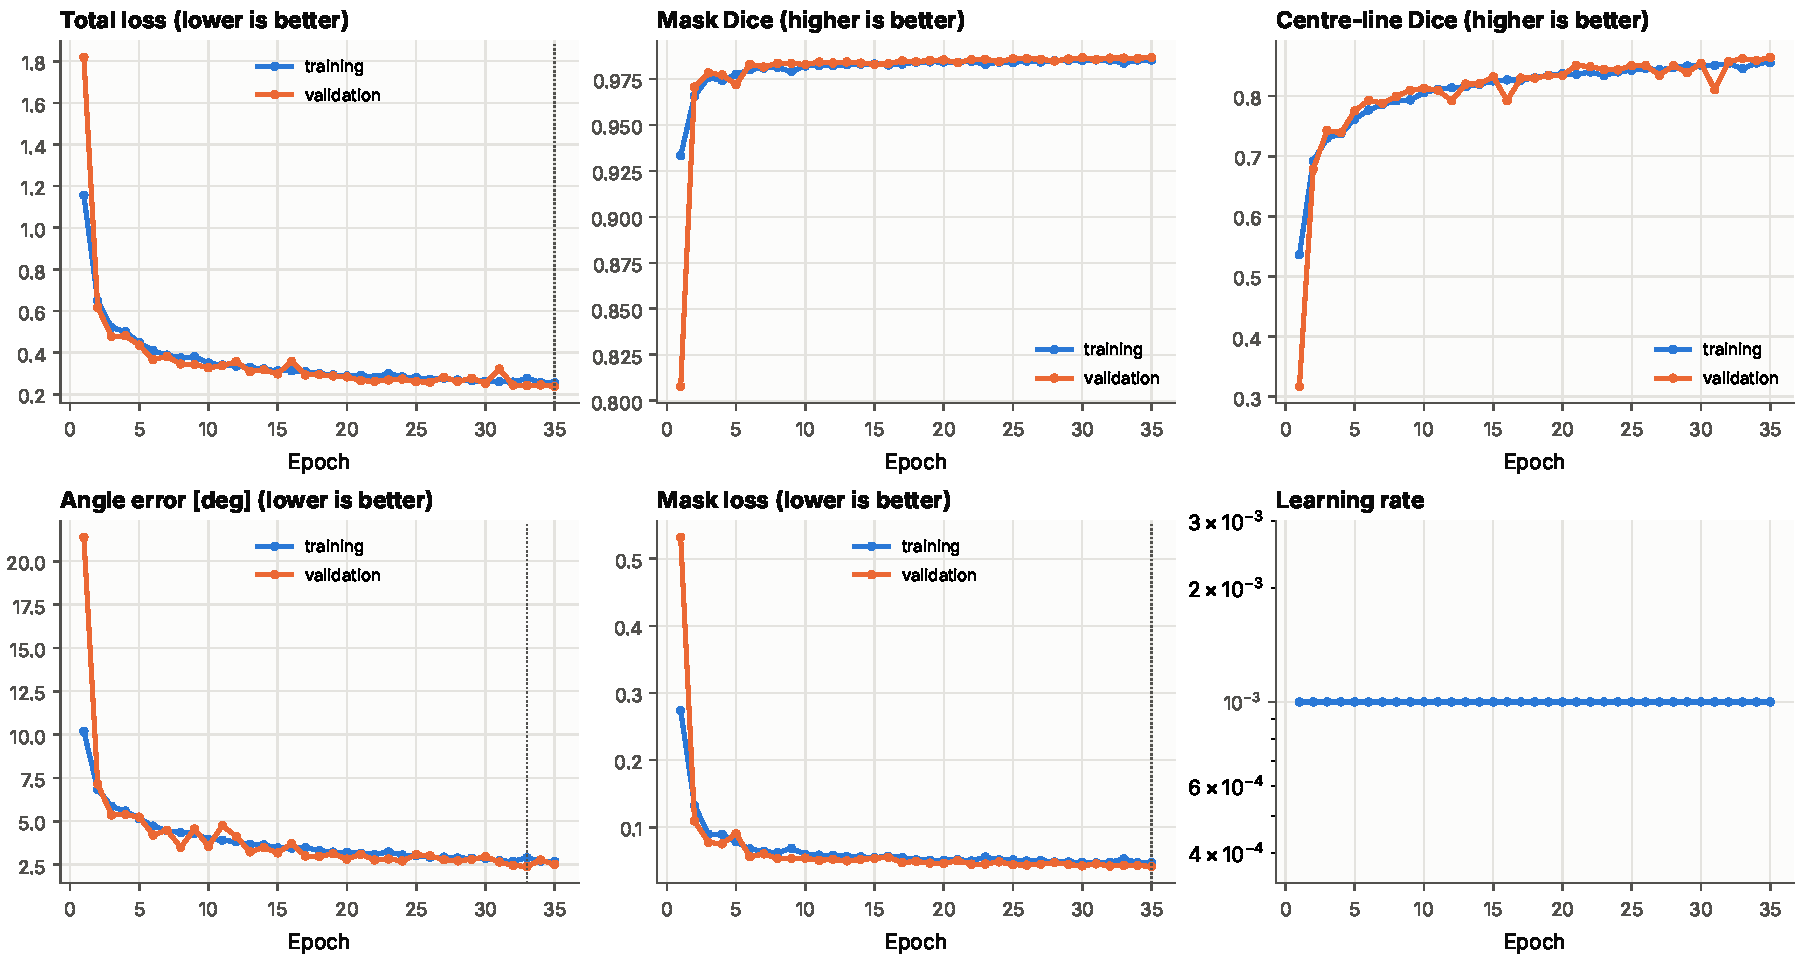
\includegraphics[width=\linewidth]{figures/training_curves.pdf}
\caption{Training of the shipped network: training (blue) and validation (orange) curves. The validation loss follows the training loss closely, so there is no generalisation gap.}\label{fig:curves}
\end{figure}

The complete pipeline (tiling, TTA, wire separation, measurement) was evaluated on two independent sets of full-size $768^2$ test images. Set A has the full density range of the training generator (coverage 7--80\,\%); set B has realistic moderate densities (coverage 4--44\,\%).

\begin{table}[H]\centering\small
\caption{Accuracy of the complete chain. Per-wire errors refer to wires matched to the ground truth; length errors to \emph{complete} wires. Per-image biases compare the statistics a user would report for one image with the truth (median over images of the absolute bias).}\label{tab:results}
\begin{tabular}{@{}lccc@{}}\toprule
 & A: all & A: coverage $\le30\,\%$ & B: moderate \\\midrule
Images & 12 & 5 & 16 \\
Mask Dice / IoU & 0.985 / 0.970 & -- & 0.982 / 0.966\\
Centre-line Dice & 0.859 & -- & 0.924 \\
Orientation error & $2.7^\circ$ & -- & $1.8^\circ$ \\
Crossings resolved & 82\,\% & -- & 93\,\% \\\midrule
Length: median rel.\ error (per wire) & $+0.07\,\%$ & $+0.24\,\%$ & $+0.37\,\%$\\
Length: within $\pm10\,\%$ & 85\,\% & 92\,\% & 92\,\% \\
Width: median rel.\ error (per wire) & $-0.46\,\%$ & $-0.29\,\%$ & $-0.70\,\%$\\
Width: within $\pm10\,\%$ & 77\,\% & 86\,\% & 92\,\% \\\midrule
Per image: $|$bias$|$ of median length & 20\,\% & 9.0\,\% & 4.4\,\% \\
Per image: $|$bias$|$ of stereological $\langle L\rangle$ & 29\,\% & 9.1\,\% & 10\,\% \\
Per image: $|$bias$|$ of median width & 2.5\,\% & 3.3\,\% & 1.2\,\% \\\bottomrule
\end{tabular}
\end{table}

\begin{figure}[H]\centering
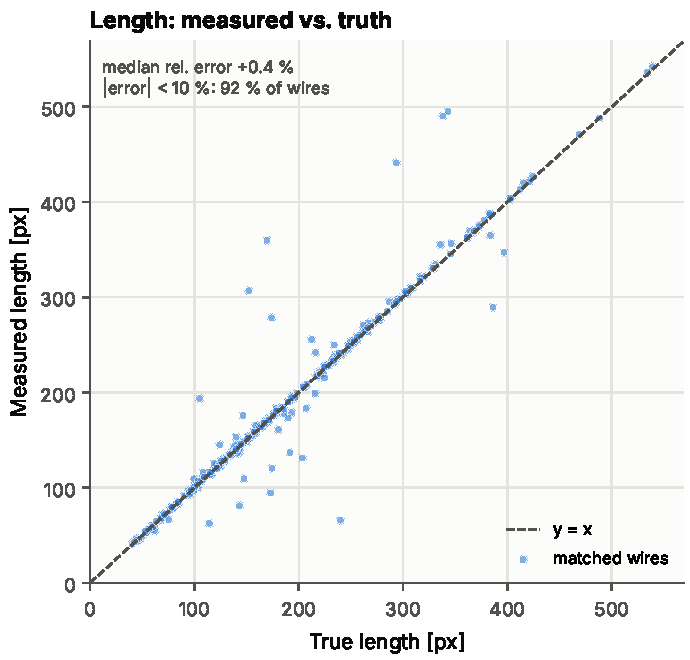
\includegraphics[width=0.45\linewidth]{figures/parity_length.pdf}\hfill
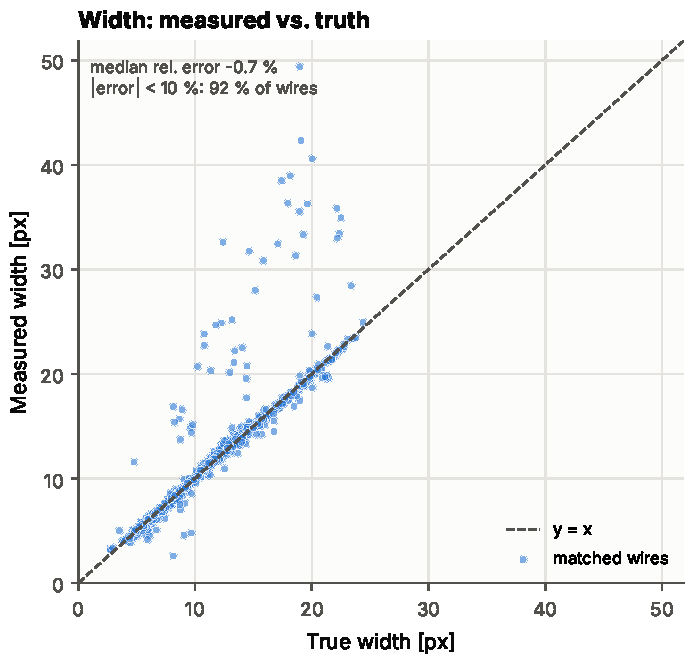
\includegraphics[width=0.45\linewidth]{figures/parity_width.pdf}
\caption{Measured vs.\ true length (complete wires) and width (all matched wires) on test set B.}\label{fig:parity}
\end{figure}

\paragraph{Interpretation.} Individual wires are measured essentially without bias: median errors are below 1\,\% for both length and width. At moderate density, the per-image deviations of the median length (typically 4\,\%, at most 14\,\%) are consistent with pure sampling noise. With $n\approx20$ complete wires from a log-normal population with $\sigma\approx0.45$, the standard error of the median is $\approx1.25\,\sigma/\sqrt n\approx12\,\%$. This is why the software always reports bootstrap confidence intervals, and why several images per sample should be analysed.

\paragraph{The physical limit: dense meshes.} Above roughly 40\,\% areal coverage most wire ends lie underneath other wires and cannot be observed, by this software or by a human. Complete wires then become rare (fewer than 35 in a $768^2$ image) and preferentially short, because a long wire crosses more wires and is more likely to lose an end ($P(\text{complete})\propto p^{k}$ for $k$ crossings resolved with probability $p$). The stereological estimator also degrades, because hidden ends are not counted. The width remains reliable at all densities (per-image bias $\le5\,\%$ up to 80\,\% coverage). The software therefore reports the coverage and a reliability class for every image (Section~\ref{sec:stats}). For length measurements on dense meshes, use images at \emph{lower} magnification, in which whole wires are visible, and keep the high-magnification images for the width.

\subsection{Stage 2: dense three-dimensional meshes and real micrographs}\label{sec:dense}
The first real micrographs supplied by the user (in-lens detector, 1\,kV, 61 and 80\,kX) showed thick, chaotic 3-D meshes with almost 100\,\% coverage. The stage-1 network traced them only in fragments. Four changes, each tested, led to the shipped network \code{models/aunw\_dense\_f16}:
\begin{enumerate}[leftmargin=*,itemsep=1pt]
\item the \code{dense3d} generator style (Section~\ref{sec:dense3d});
\item the width head (Sections~\ref{sec:targets} and~\ref{sec:measure});
\item \textbf{visible-only labels}. This was the decisive change. With labels that included hidden centre-lines, even \emph{perfect} maps gave a wire continuity of only 0.33. Continuity is the length-weighted fraction of a true wire's visible centre-line covered by a single detected wire. Visible-only labels raised it to 0.76 on perfect maps and from 0.28 to 0.56 for the network;
\item a capped automatic scale. Enlarging images by more than about $1.5\times$ made interpolated noise look like fine wires (hundreds of phantom wires), so the image is now only shrunk freely and enlarged by at most $1.5\times$, and the software warns when wires are narrower than about 5\,px.
\end{enumerate}
Training started from the stage-1 weights (transfer learning) and ran for 30 epochs on 2000 tiles (about 2\,h on 4 CPU cores). Training and validation loss stayed together; the best epoch was the last one.

\begin{table}[H]\centering\small
\caption{Shipped network on 12 dense synthetic $768^2$ images (coverage 55--97\,\%), compared with width from edge profiles.}\label{tab:dense}
\begin{tabular}{@{}lc@{}}\toprule
Mask Dice / centre-line Dice / orientation error & 0.955 / 0.744 / $6.9^\circ$ \\
Width (width map): median error per wire & $-0.9\,\%$ \\
Width (width map): wires within $\pm10\,\%$ & \textbf{85\,\%} \\
Width (edge profiles): wires within $\pm10\,\%$ & 27\,\% \\
Per image: $|$bias$|$ of the median width & 2.7\,\% \\
Complete wires (length measurable) & 4 in 12 images \\\bottomrule
\end{tabular}
\end{table}

\paragraph{Real micrographs.} On the two real images the network traces most visible wires as single wires across the field (Fig.~\ref{fig:real}). Correctly, almost none is classified as complete: nearly all wires leave the field of view, so their length cannot be measured from these images. The median widths are 150.7\,nm (61\,kX, 8.33\,nm/px, IQR 139--163\,nm) and 144.2\,nm (80\,kX, 6.38\,nm/px, IQR 130--157\,nm). Two images at different magnifications, and therefore different pixel sizes, agree within 4.5\,\%, which is a consistency check of the calibration and of the scale invariance. The edge-profile width gives 262 and 242\,nm on the same images: in a dense mesh the cross-section runs into touching wires, as predicted. Calibration was taken from the scale bar of screenshots; with the original TIFF files the pixel size is read from the metadata.

\begin{figure}[H]\centering
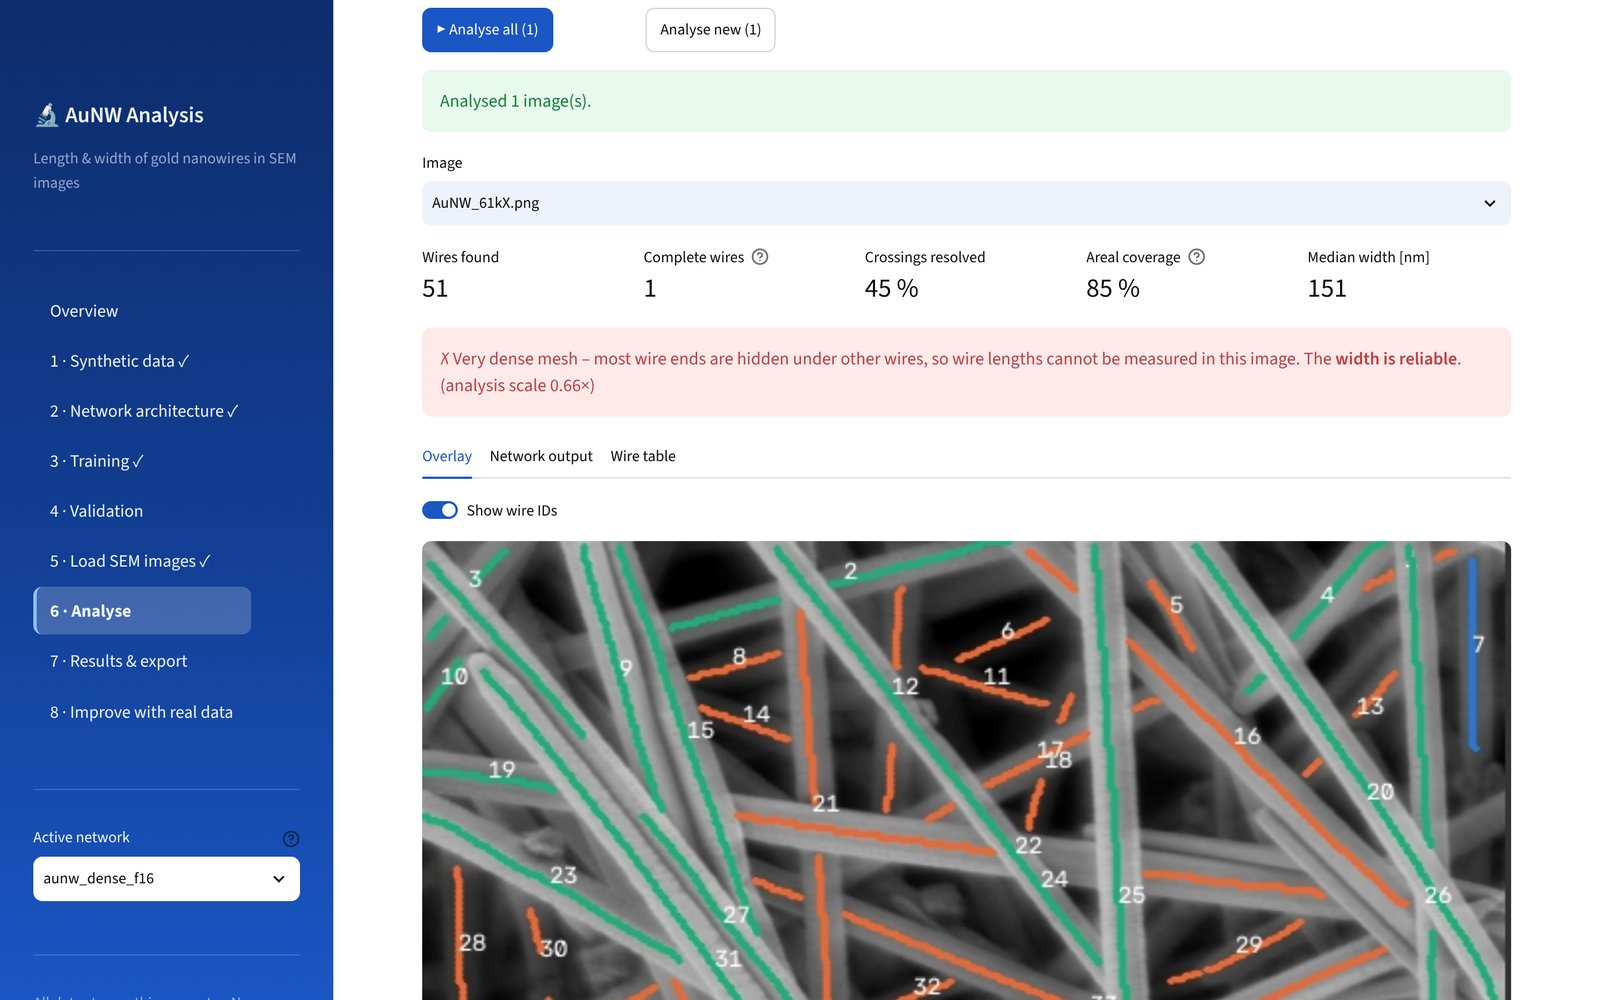
\includegraphics[width=\linewidth]{figures/ui_analyse_real.jpg}
\caption{Analysis of a real micrograph (step 6). Green: wires traced across the field and cut by the border (width only); orange: wires ending in a crossing (width only). The reliability check correctly reports that lengths cannot be measured in this image.}\label{fig:real}
\end{figure}

\paragraph{Recommended measurement protocol.} (i) Width: high-magnification images such as these (wire width $\gtrsim10$\,px), several images per sample. (ii) Length: images at a magnification low enough that whole wires, including both tips, are visible and coverage is below about 30\,\%. (iii) Check a few wires against manual measurements (step 4) and, if needed, fine-tune with 3--5 corrected masks (step 8).

\paragraph{Design alternatives that were tested and rejected.} Reporting these is part of good scientific practice:
\begin{itemize}[leftmargin=*,itemsep=1pt]
\item \emph{Junction contraction} (merging junctions joined by short branches, intended for shallow-angle crossings) reduced the fraction of wires within $\pm10\,\%$ from 71\,\% to 60\,\% and was removed.
\item \emph{Counting T-ends as complete} raised the number of usable wires but admitted 26--62\,\% fragments.
\item \emph{Gap bridging} (Section~\ref{sec:graph}) brought only a small gain in stage 1 (crossings resolved 79\,\%$\to$82\,\%). With the visible-only labels of stage 2 it became the mechanism that follows a lower wire through every crossing.
\item \emph{Horvitz--Thompson weights $p^{-k}$} for the survivorship bias, with $p$ estimated per image (globally or per junction degree), over-corrected the mean by $+36$ to $+57\,\%$ because $p$ is strongly heterogeneous, and was not adopted.
\end{itemize}

%==========================================================================
\section{Improving the network with real SEM images}\label{sec:finetune}
%==========================================================================
The synthetic renderer is an approximation of reality, so a residual \emph{domain gap} is expected. The software provides a closed improvement loop:
\begin{enumerate}[leftmargin=*,itemsep=1pt]
\item Analyse a real micrograph (step 6) and download the predicted mask.
\item Correct the mask in ImageJ/Fiji or GIMP (white = wire). Correcting is much faster than drawing from scratch.
\item Upload image and mask pairs in step 8. Images are rescaled with the same automatic scale as in the analysis, then cut into tiles. The centre-line target is derived from the skeleton of the mask; the orientation weight is set to zero, since real data teach mask and centre-line, while synthetic data keep teaching orientation.
\item Fine-tune with the \textbf{encoder frozen} (general features are kept and only the decoder adapts), a small learning rate ($10^{-4}$), and every batch a fixed mixture of real and synthetic tiles (default 50/50). Mixing prevents \emph{catastrophic forgetting} of the synthetic knowledge. Early stopping monitors the loss on \emph{held-out real images}.
\item Compare old and new networks in step 4: Dice on annotated real images, or agreement with manual measurements via the KS test.
\end{enumerate}
The train/validation split for real data must be made \emph{by image, never by tile}. Neighbouring tiles of one micrograph share wires, illumination and noise, so a tile-wise split would leak information and the validation loss would be over-optimistic.

%==========================================================================
\section{Using the software}
%==========================================================================
On Windows, \code{install\_windows.bat} installs everything once and creates a desktop and start-menu shortcut with the program icon, a beaker filled with gold nanowires (\code{tools/make\_icon.py} draws it). Clicking it runs \code{desktop.py}, which starts the analysis server invisibly on a free local port and shows the interface in a native window (pywebview with the Edge WebView2 engine; fallback: Edge or Chrome in app mode, without tabs or address bar). Closing the window stops everything. On other systems: \code{python desktop.py}, or \code{streamlit run app.py} for the browser version. The blue column on the left lists the steps; completed steps are marked with \checkmark. The active network is selected at the bottom of the column. For routine analysis only steps 5--7 are needed:
\begin{description}[leftmargin=1.2em,itemsep=1pt]
\item[Step 5] Upload TIFF/JPEG/PNG files, or read a whole folder. Check the cropped information bar and the calibration (metadata, nm/px or scale bar). The calibration of the first image can be applied to all.
\item[Step 6] Run the analysis. The overlay colours complete wires blue, wires ending in a crossing orange, and wires cut by the border green. Tabs show the raw network output and the table of all wires.
\item[Step 7] Choose the unit and the edge correction. The page shows the summary table, histograms with normal and log-normal fits, length vs.\ width, per-image box plots and CDFs. Downloads: CSV, Excel (sheets \emph{Summary}, \emph{Wires}, \emph{Per image}, \emph{Settings}), each figure as PNG (300\,dpi), SVG or PDF, and a ZIP of everything, including overlays and the exact analysis settings for reproducibility.
\end{description}
Headless use, for example training on a GPU server, is possible with \code{python -m aunw.cli} and the sub-commands \code{generate}, \code{train}, \code{finetune}, \code{evaluate} and \code{analyze}. All processing is local: the server listens only on \code{localhost} and usage statistics are disabled.

\subsection*{Screenshots}
\begin{figure}[H]\centering
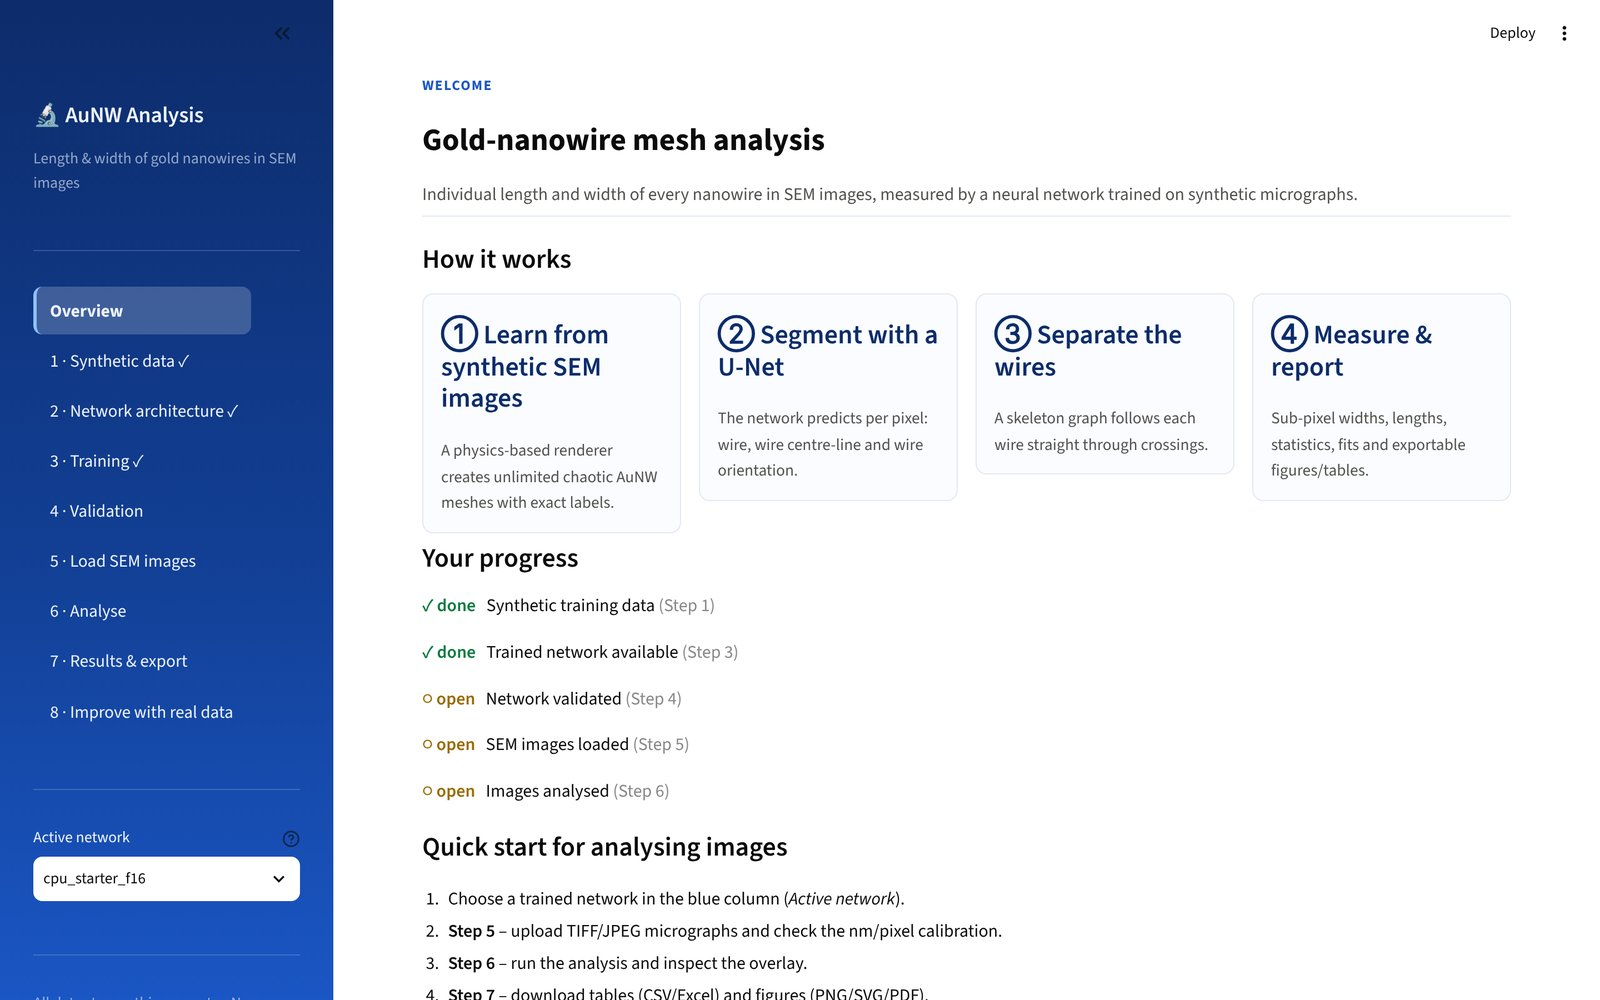
\includegraphics[width=0.49\linewidth]{figures/ui_overview.jpg}\hfill
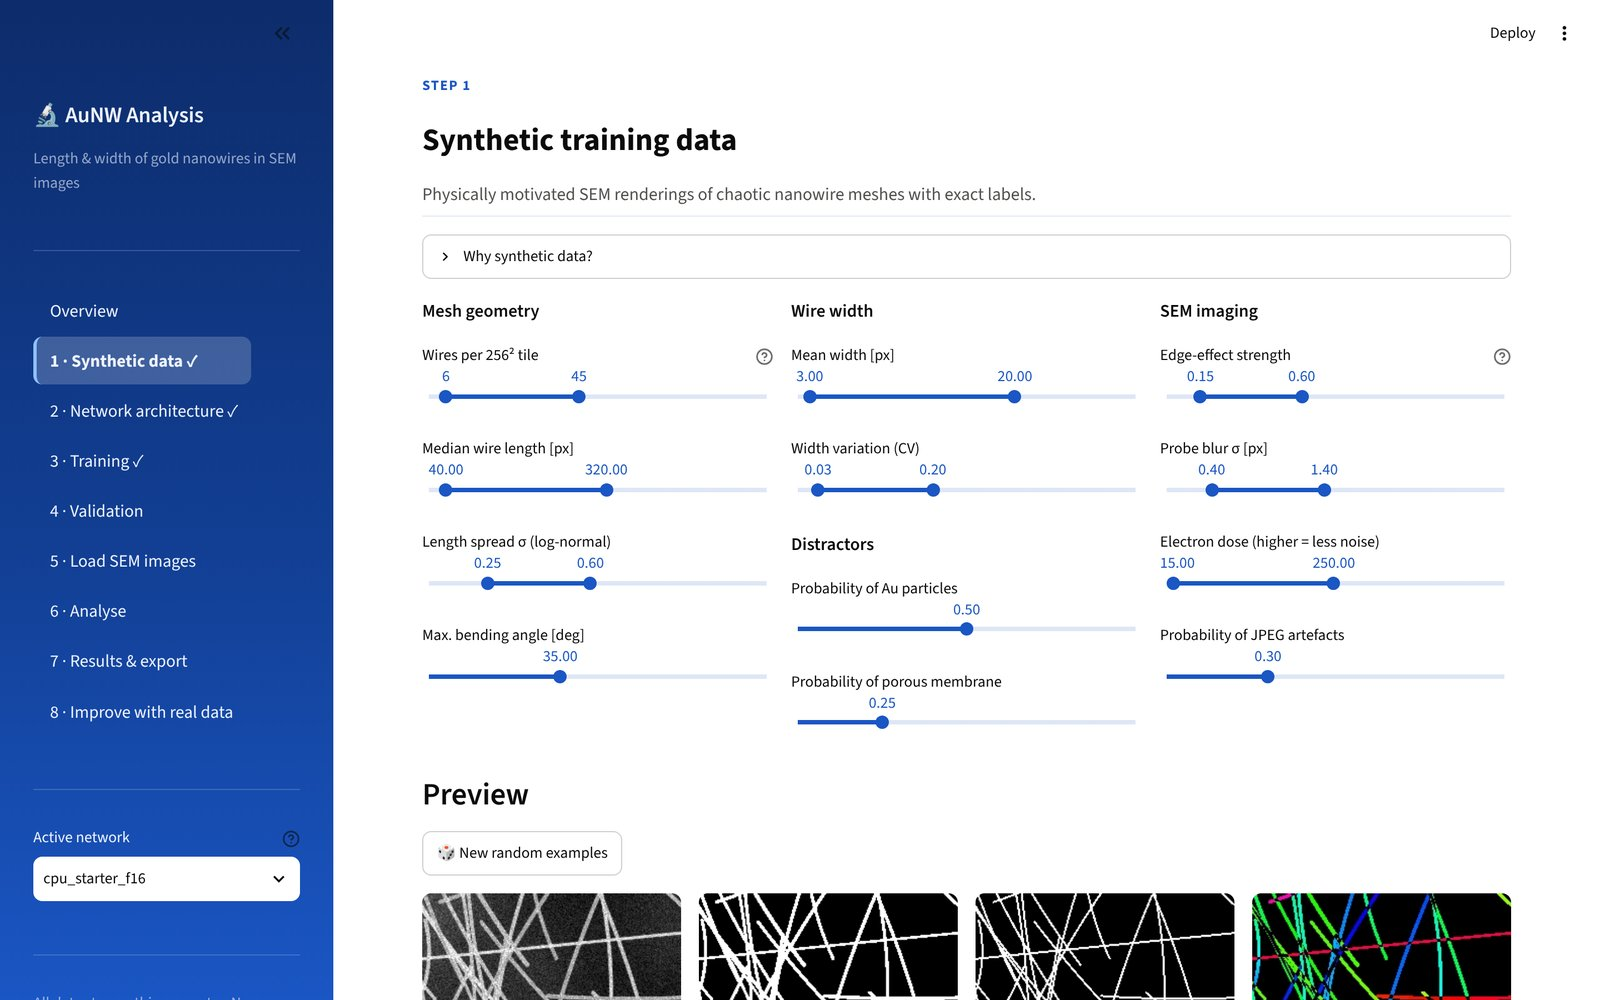
\includegraphics[width=0.49\linewidth]{figures/ui_synthetic.jpg}\\[4pt]
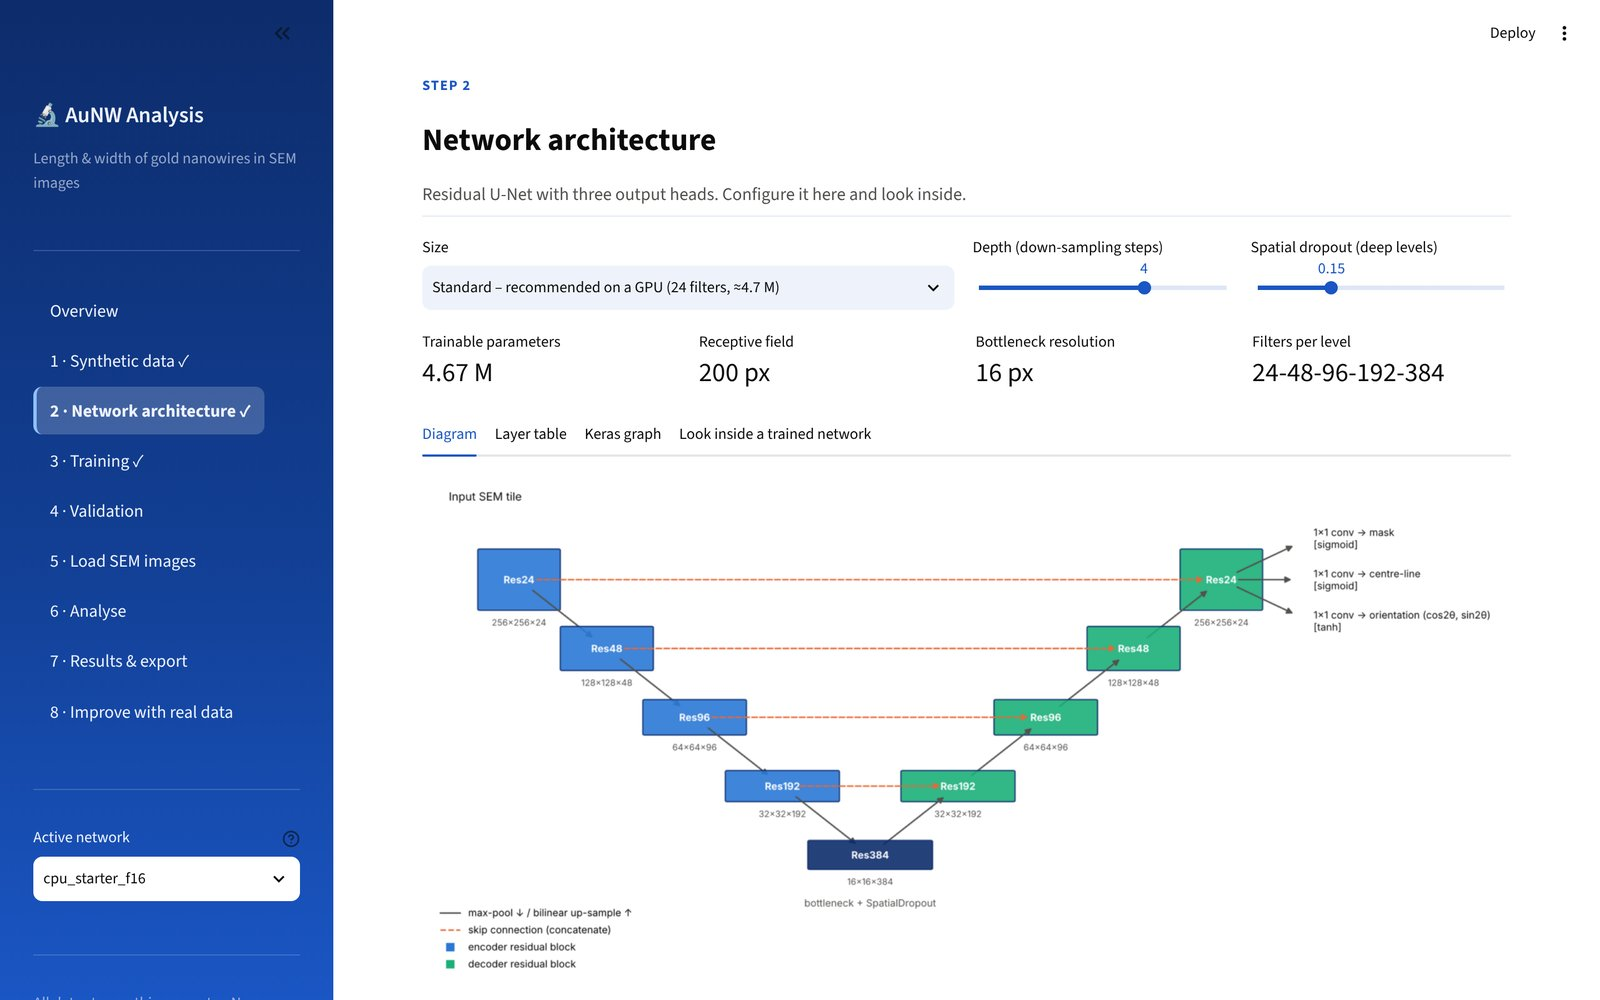
\includegraphics[width=0.49\linewidth]{figures/ui_network.jpg}\hfill
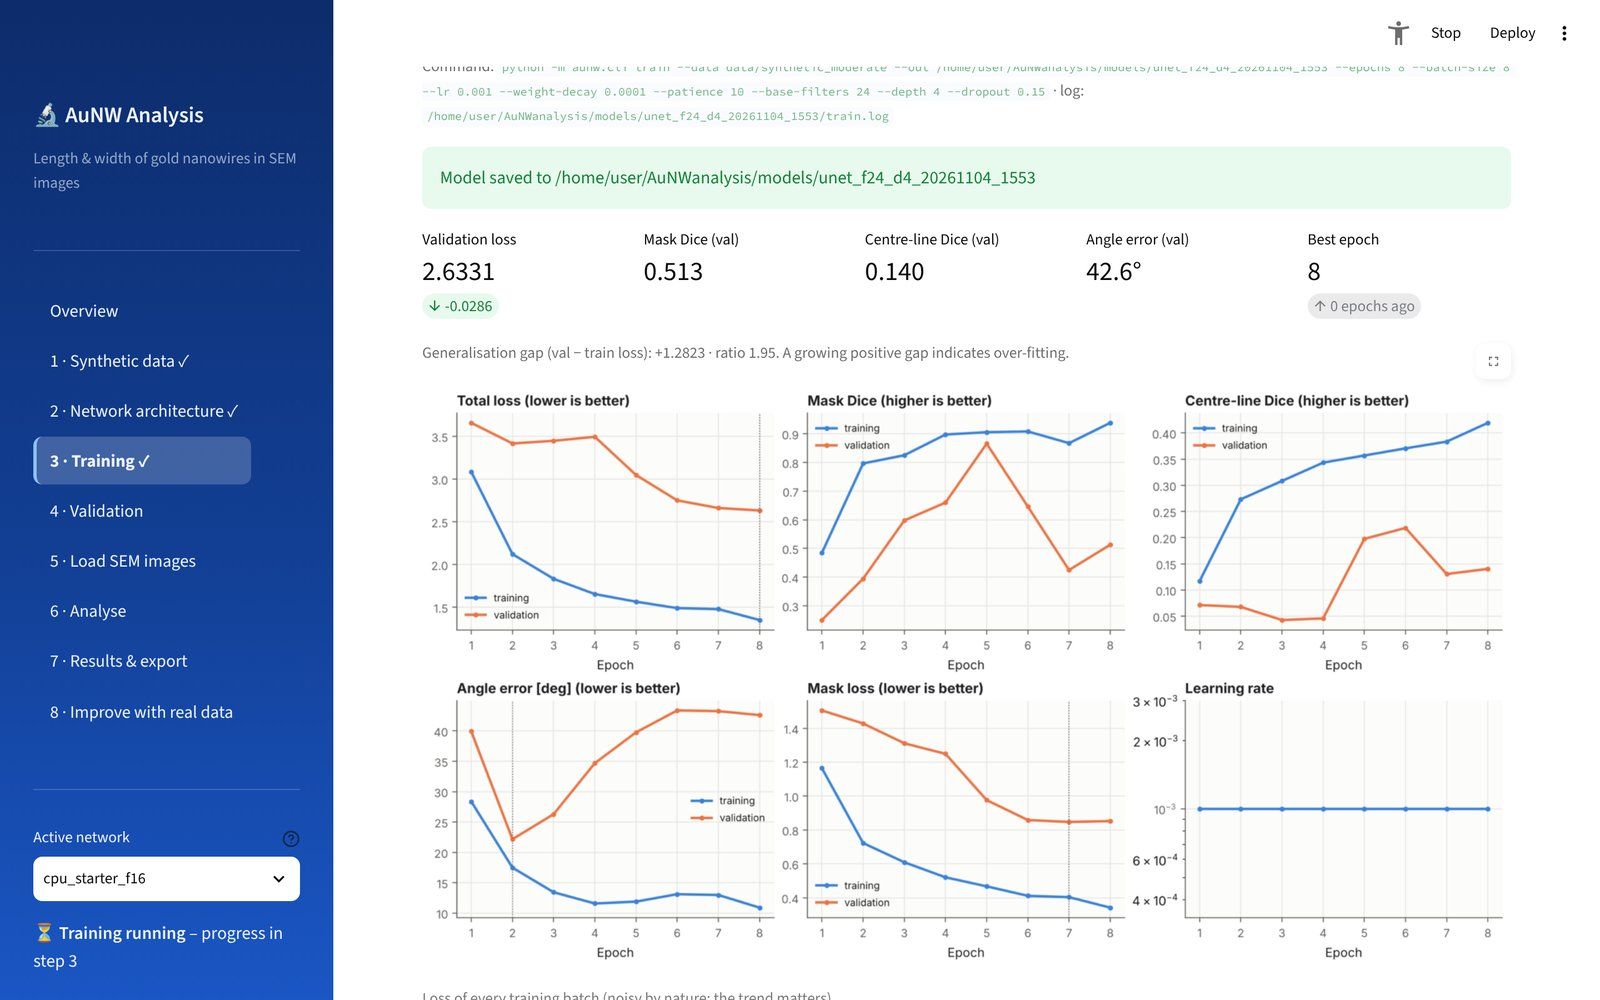
\includegraphics[width=0.49\linewidth]{figures/ui_training.jpg}
\caption{Overview, synthetic data generator (step 1), network architecture (step 2) and live training monitor (step 3, shown here for a deliberately tiny training set, so the over-fitting gap is visible).}
\end{figure}
\begin{figure}[H]\centering
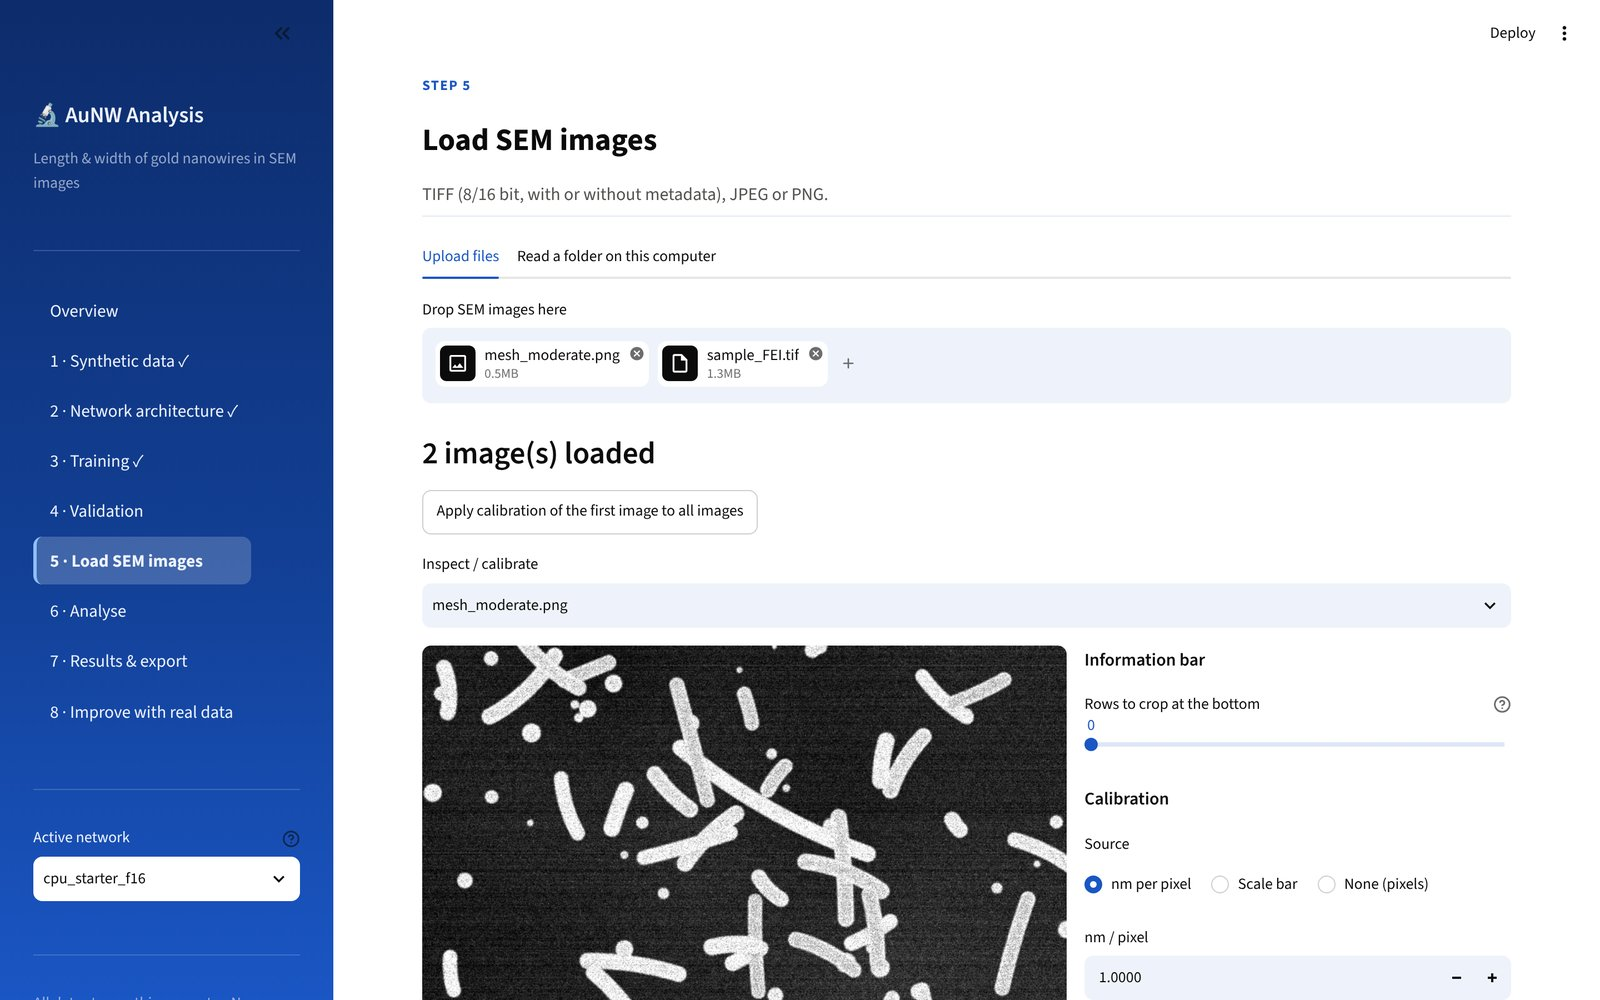
\includegraphics[width=0.49\linewidth]{figures/ui_load.jpg}\hfill
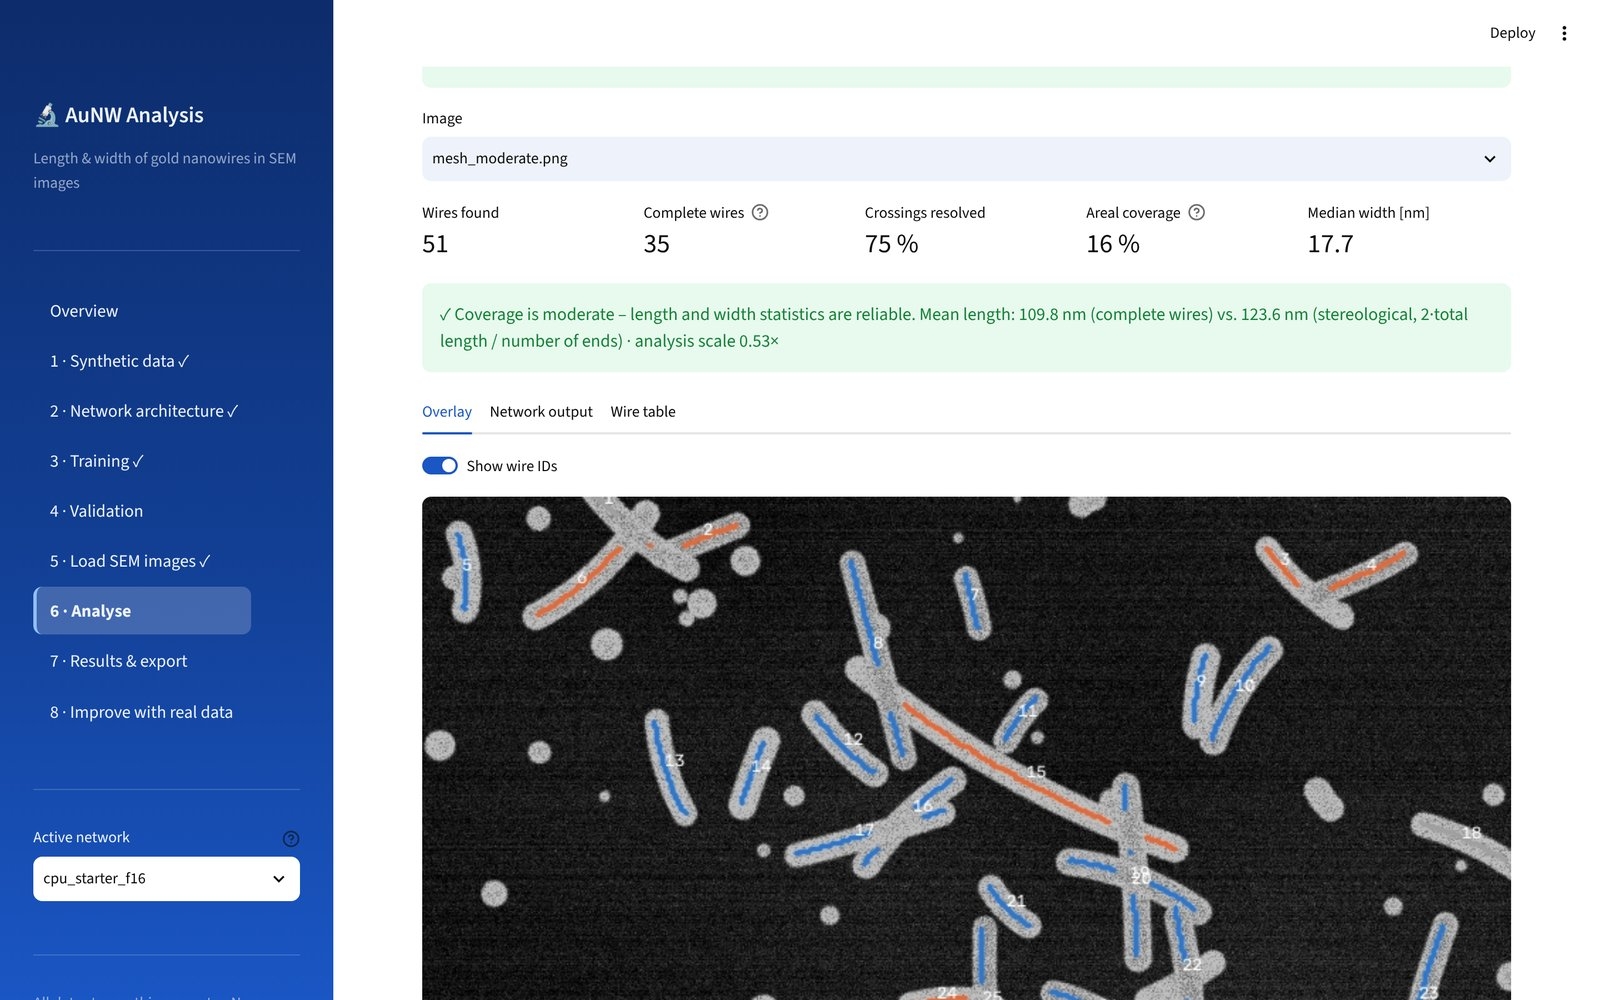
\includegraphics[width=0.49\linewidth]{figures/ui_analyse.jpg}\\[4pt]
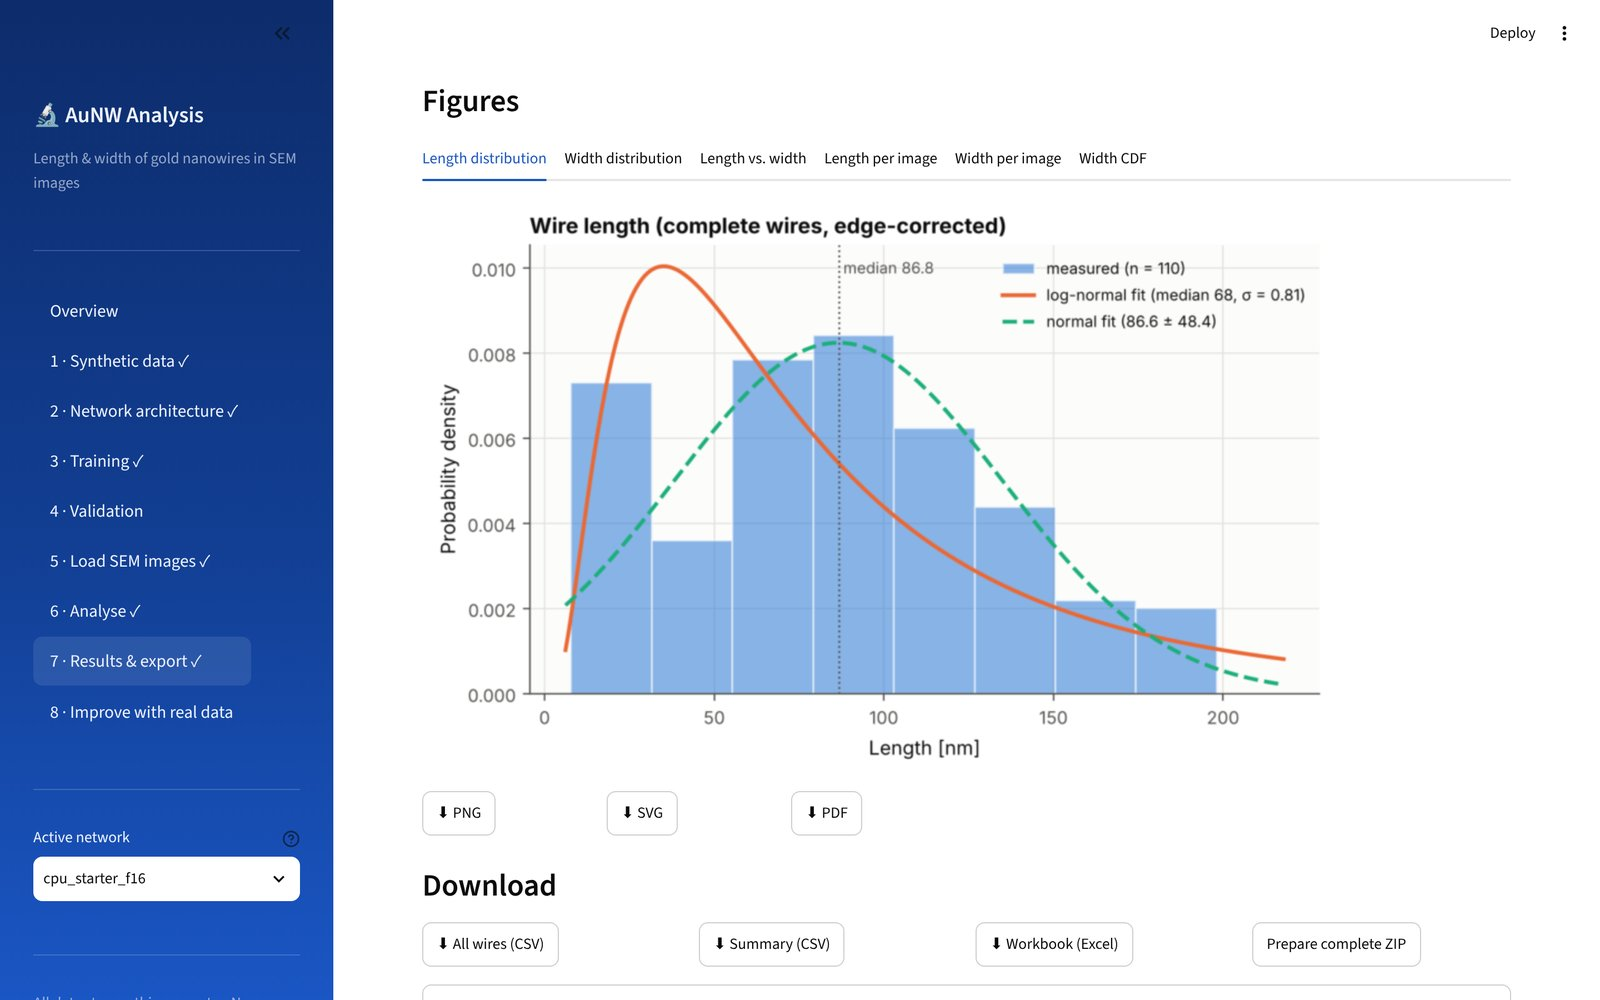
\includegraphics[width=0.49\linewidth]{figures/ui_results.jpg}
\caption{Loading and calibrating images (step 5), analysis with overlay, coverage-based reliability check and the two mean-length estimates (step 6), and results with fitted distributions and exports (step 7).}
\end{figure}


%==========================================================================
\section{Proposed additional features (for discussion)}
%==========================================================================
The current version focuses on length and width, as agreed. The following quantities can be derived from the existing graph and maps with little extra effort and are relevant for AuNW networks such as transparent electrodes:
\begin{enumerate}[leftmargin=*,itemsep=1pt]
\item \textbf{Orientation distribution and order parameter} $S=|\langle e^{2i\theta}\rangle|$ ($0$ isotropic, $1$ aligned), relevant for anisotropic conductivity.
\item \textbf{Wire density} $n$ (wires per \si{\micro m^2}) and \textbf{areal coverage}. Together with $\langle L\rangle$ they give the stick-percolation parameter $nL^2$, to be compared with the threshold $n_cL^2\approx5.64$~\cite{li2009}.
\item \textbf{Junction density and coordination number} (contacts per wire), which govern the junction-resistance-dominated sheet resistance.
\item \textbf{Pore-size distribution} of the mesh (sizes of background regions enclosed by wires), relevant for optical transmittance and haze.
\item \textbf{Curvature and tortuosity} $\tau=L/\text{end-to-end distance}$ for flexible ultrathin wires.
\item \textbf{Width uniformity along a wire} (tapering, necking), from the individual profile widths $w_i$ that are already computed.
\item \textbf{By-product analysis}: count and size distribution of Au particles, and the yield (wire area / total Au area).
\item \textbf{Bundles}: detection of parallel touching wires from width outliers and orientation.
\end{enumerate}

\begin{thebibliography}{9}\small
\bibitem{ronneberger2015} O.~Ronneberger, P.~Fischer, T.~Brox. U-Net: Convolutional networks for biomedical image segmentation. \emph{MICCAI} (2015).
\bibitem{he2016} K.~He, X.~Zhang, S.~Ren, J.~Sun. Deep residual learning for image recognition. \emph{CVPR} (2016).
\bibitem{odena2016} A.~Odena, V.~Dumoulin, C.~Olah. Deconvolution and checkerboard artifacts. \emph{Distill} (2016).
\bibitem{loshchilov2019} I.~Loshchilov, F.~Hutter. Decoupled weight decay regularization. \emph{ICLR} (2019).
\bibitem{miles1978} R.~E.~Miles. The sampling, by quadrats, of planar aggregates. \emph{J.~Microsc.} 113, 257 (1978).
\bibitem{lantuejoul1980} C.~Lantuéjoul. On the estimation of mean values in individual analysis of particles. \emph{Microsc.\ Acta} 5, 266 (1980).
\bibitem{li2009} J.~Li, S.-L.~Zhang. Finite-size scaling in stick percolation. \emph{Phys.\ Rev.\ E} 80, 040104 (2009).
\bibitem{reimer} L.~Reimer. \emph{Scanning Electron Microscopy}, 2nd ed., Springer (1998).
\end{thebibliography}
\end{document}
